\documentclass[letterpaper, 12pt]{article}
% \usepackage[showframe, margin=1in, top=0.25in, bottom=0.25in, includeheadfoot, headheight=0.5in]{geometry}
\usepackage[margin=1in, top=0.25in, bottom=0.25in, includeheadfoot, headheight=0.5in]{geometry}

\AddToHook{cmd/section/before}{\clearpage}

\usepackage[table]{xcolor}
\colorlet{listingback}{gray!20}
\definecolor{headingcolor}{RGB}{110,34,54}

\usepackage{fancyhdr}
\renewcommand{\sectionmark}[1]{\markboth{#1}{#1}}

% Used to detect whether a section is an appendix to print the right thing in the footer
\usepackage{etoolbox}
\newtoggle{inappendix}
\pretocmd{\appendix}{\clearpage\toggletrue{inappendix}}{}{}

% Save standard definitions for head and foot rules (lines separating header and footer from text)
\let\HeadRule\headrule
\let\FootRule\footrule
% Add color to the standard definitions
\renewcommand{\headrule}{\color{headingcolor}\HeadRule}
\renewcommand{\footrule}{\textcolor{headingcolor}{\FootRule}}

% IMPORTANT: This command should not be called directly. Use \preamble.
% Macro to insert the title page for each lab.
% The argument is the title of the lab.
\newcommand{\inserttitlepage}[1]
{
    \begin{titlepage}
    \centering
    
\includegraphics[scale=0.5]{images/nexus_lab_logo.png}

    \vspace*{\baselineskip}

    \textbf{\Large OpenStack Labs}

    \vspace*{\baselineskip}

    \textbf{\Large #1}
    \vspace*{\fill}
\end{titlepage}
}

% IMPORTANT: This command should not be called directly. Use \preamble.
% Macro to define header and footer for each lab.
% The argument is the title of the lab.
\newcommand{\headfoot}[1]
{
    \fancypagestyle{fancy}
    {
        \fancyhf{}
        \fancyhead[L]{\footnotesize #1}
        \fancyhead[R]{
\includegraphics[height=0.85\headheight]{images/nexus_lab_logo.png}}
        \fancyfoot[L]{%
            \footnotesize%
            \ifnum\value{section}>0%
            \iftoggle{inappendix}{Appendix \thesection: \rightmark}{Section \thesection: \rightmark}%
            \fi}
        \fancyfoot[R]{\footnotesize\thepage}
        \renewcommand{\headrulewidth}{1.5pt}
        \renewcommand{\footrulewidth}{1.5pt}
    }
}

% Macro to insert title page, define header and footer, and insert table of contents and about section for each lab.
% The argument is the title of the lab.
\newcommand{\preamble}[1]
{
    \pagenumbering{roman}
    \inserttitlepage{#1}
    \headfoot{#1}

    % Insert table of contents
    \pagestyle{fancy}
    \tableofcontents
    \clearpage

    \section*{About This Document}
    \label{sec:about_this_document}
    \begin{itemize}
        \item This document was developed by a team at the University of Tennessee at Chattanooga led by Dr. Mengjun Xie
        (\href{mailto:mengjun-xie@utc.edu}{\textbf{mengjun-xie@utc.edu}}).
        \item The development of this document was supported by a National Centers of Academic Excellence in Cybersecurity Grant (\#H98230-20-1-0351), housed at the National Security Agency.
        \item This document is licensed with a Creative Commons Attribution 4.0 International License.
    \end{itemize}
    \clearpage
}

% Macro to insert the Lab Settings page for each lab. Call after the Introduction and Objectives sections.
\newcommand{\labsettings}
{
    \section*{Lab Settings}
    \label{sec:lab_settings}
    \addcontentsline{toc}{section}{\nameref{sec:lab_settings}}
    The information in the table below will be needed in order to complete the lab.
    The task sections below provide details on the use of this information.
    \begin{table*}[htbp]
        \centering
        \begin{tabular}{|c|c|c|c|}
            \hline
            \rowcolor{gray!20} \textbf{Virtual Machine} & \textbf{IP Address} & \textbf{Account} & \textbf{Password} \\
            \hline
            \multirow{2}{*}{\texttt{workstation}} & \multirow[t]{2}{*}{\texttt{ens3: 192.168.1.21}}  & \multirow{2}{*}{\texttt{ubuntu}} & \multirow{2}{*}{\texttt{ubuntu}} \\
                                                  & \multirow[t]{2}{*}{\texttt{ens4: 172.25.250.21}} &                                  &                                  \\
            \hline
            \multirow{2}{*}{\texttt{devstack}}    & \multirow[t]{2}{*}{\texttt{ens3: 192.168.20}}    & \multirow{2}{*}{\texttt{ubuntu}} & \multirow{2}{*}{\texttt{ubuntu}} \\
                                                  & \multirow[t]{2}{*}{\texttt{ens4: 172.25.250.20}} &                                  &                                  \\
            \hline
        \end{tabular}
    \end{table*}
    \clearpage

    % IMPORTANT(lucas): If another frontmatter section ever gets placed after this, this command needs to be moved
    % to the end of that section.
    % I have placed this here and not in each lab purely for convenience and to ensure I don't forget any.
    \pagenumbering{arabic}
}

% Sans-serif font
\renewcommand{\familydefault}{\sfdefault}
\newcommand{\texttildemid}{{\raisebox{0.5ex}{\texttildelow}}}

\usepackage{enumitem}
\renewcommand{\labelenumi}{\textbf{\thesection.\arabic{enumi}.}}

% Try to forbid widows and orphans
\widowpenalty10000
\clubpenalty10000

\usepackage{graphicx}
\usepackage{hyperref}
\hypersetup{colorlinks=true,linkcolor=black,urlcolor={[named] headingcolor}}

\usepackage{sectsty}
\sectionfont{\color{headingcolor}}

% Table of Contents
\usepackage{bookmark}
\usepackage[titles]{tocloft}
\usepackage[title]{appendix}
\renewcommand{\cfttoctitlefont}{\Large\bfseries\color{headingcolor}}
\renewcommand{\cftsecfont}{\normalfont\normalsize}
\renewcommand{\cftsecpagefont}{\normalfont\normalsize}
\renewcommand{\cftdotsep}{0} % Make dots small and close together
\renewcommand{\cftsecleader}{\cftdotfill{\cftdotsep}} % Add dots after section titles
% Make dots go all the way to the page number
\renewcommand{\cftsecfillnum}[1]{{\cftsecleader}\nobreak{\cftsecpagefont #1}\cftsecafterpnum\par}

\usepackage{multirow}
\setlength{\tabcolsep}{16pt}
\renewcommand{\arraystretch}{1.1}

% For nice-looking boxes
\usepackage[most]{tcolorbox}
\usepackage{listings}
\usepackage{lstautogobble}
\lstset{
  frame=none,
  language=Bash,
  showstringspaces=false,
  basicstyle={\linespread{1.1}\footnotesize\ttfamily\selectfont},
  numbers=none,
  breaklines=true,
  breakatwhitespace=true,
  tabsize=3,
  columns=fullflexible,
  keepspaces=true,
  escapeinside={(*@}{@*)},
  literate={~}{{\texttildemid}}{1}
           {\#}{\#}{1},
  autogobble=true
}

\tcolorboxenvironment{lstlisting}
{
    spartan,
    colframe=gray!50,
    boxsep=0mm,
    left=1mm,
    right=1mm,
    top=-1mm,
    bottom=-1mm,
    colback=gray!20
}

% Hacky solution for now, would like to have just one environment and make several tcolorboxes by passing different
% colors as parameters, but that is giving errors
\makeatletter
\tcbset{
  note/.style={%
        enhanced,
        breakable,
        colback=blue!10!white,
        colframe=blue!80!white,
        attach boxed title to top left={yshift*=-\tcboxedtitleheight},
        title={#1},
        boxed title size=title,
        boxed title style={%
            sharp corners,
            rounded corners=northwest,
            colback=tcbcolframe,
            boxrule=0pt,
        },
        underlay boxed title={%
            \path[fill=tcbcolframe] (title.south west)--(title.south east)
                to[out=0, in=180] ([xshift=5mm]title.east)--
                (title.center-|frame.east)
                [rounded corners=\kvtcb@arc] |-
                (frame.north) -| cycle;
        },
    }
}
\makeatother

\makeatletter
\tcbset{
    stop/.style={%
        enhanced,
        breakable,
        colback=white,
        colback=red!10!white,
        colframe=red!80!white,
        attach boxed title to top left={yshift*=-\tcboxedtitleheight},
        title={#1},
        boxed title size=title,
        boxed title style={%
            sharp corners,
            rounded corners=northwest,
            colback=tcbcolframe,
            boxrule=0pt,
        },
        underlay boxed title={%
            \path[fill=tcbcolframe] (title.south west)--(title.south east)
                to[out=0, in=180] ([xshift=5mm]title.east)--
                (title.center-|frame.east)
                [rounded corners=\kvtcb@arc] |-
                (frame.north) -| cycle;
        },
    }
}
\makeatother

\makeatletter
\tcbset{
    tip/.style={%
        enhanced,
        breakable,
        colback=white,
        colback=green!10,
        colframe=green!70!black,
        attach boxed title to top left={yshift*=-\tcboxedtitleheight},
        fonttitle=\bfseries,
        title={#1},
        boxed title size=title,
        boxed title style={%
            sharp corners,
            rounded corners=northwest,
            colback=tcbcolframe,
            boxrule=0pt,
        },
        underlay boxed title={%
            \path[fill=tcbcolframe] (title.south west)--(title.south east)
                to[out=0, in=180] ([xshift=5mm]title.east)--
                (title.center-|frame.east)
                [rounded corners=\kvtcb@arc] |-
                (frame.north) -| cycle;
        },
    }
}
\makeatother

% The commands below define environments for colored boxes. They are used like
% \begin{notebox}
% ...
% \end{notebox}
\newtcolorbox{notebox}{note={Note}}
\newtcolorbox{stopbox}{stop={Stop}}
\newtcolorbox{tipbox}{tip={Tip}}

\begin{document}
\preamble{Lab 05: Deploying an External Instance}

\section*{Introduction}\label{sec:introduction}
\addcontentsline{toc}{section}{\nameref{sec:introduction}}
In the previous lab, you created an external network, a router, and floating IP addresses.
However, you were still not able to connect to an instance connected to the external network from outside the OpenStack environment.
In this lab, you will create security groups to allow the traffic to reach the external instance, and you will create an SSH key pair so that you can remotely log in to the instance.

\section*{Objectives}\label{sec:objectives}
\addcontentsline{toc}{section}{\nameref{sec:objectives}}
\begin{itemize}[itemsep=0pt]
    \item Create and manage security groups.
    \item Create and manage SSH key pairs.
    \item Launch and verify an external instance.
\end{itemize}
\clearpage

\labsettings

%%%%%%%%%%%
% Section 1
%%%%%%%%%%%
\section{Defining Security Groups}\label{sec:defining-security-groups}
In this task, you will use the \textit{Horizon Dashboard} and \textit{OpenStack Unified CLI} to manage security groups for OpenStack instances.
Security groups function like virtual firewalls, allowing you to define rules that allow or deny specific types of network traffic.
Modifying the default security group settings is essential to enable communication with external instances from outside the OpenStack environment.
In this lab, we are concerned with two types of traffic in particular: ICMP to allow the use of the \textbf{ping} command, and SSH to enable remote login from an external network.

\begin{enumerate}
    \begin{labstep}
        Log in to the \textbf{workstation} machine as the \textbf{ubuntu} user with password \textbf{ubuntu}.

        \begin{center}
            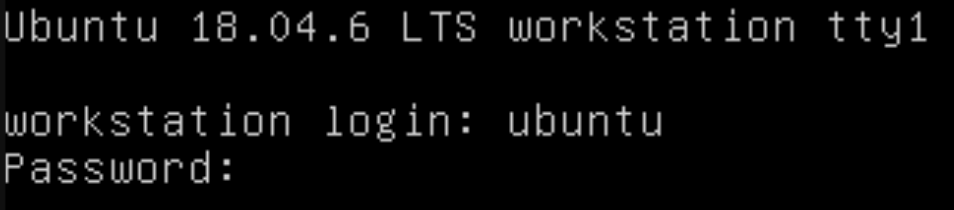
\includegraphics[width=\linewidth]{images/part1/step1.png}
        \end{center}
    \end{labstep}

    \begin{labstep}
        Launch the graphical user interface.
        \begin{lstlisting}
            ubuntu@workstation:~$ startx
        \end{lstlisting}

        \begin{center}
            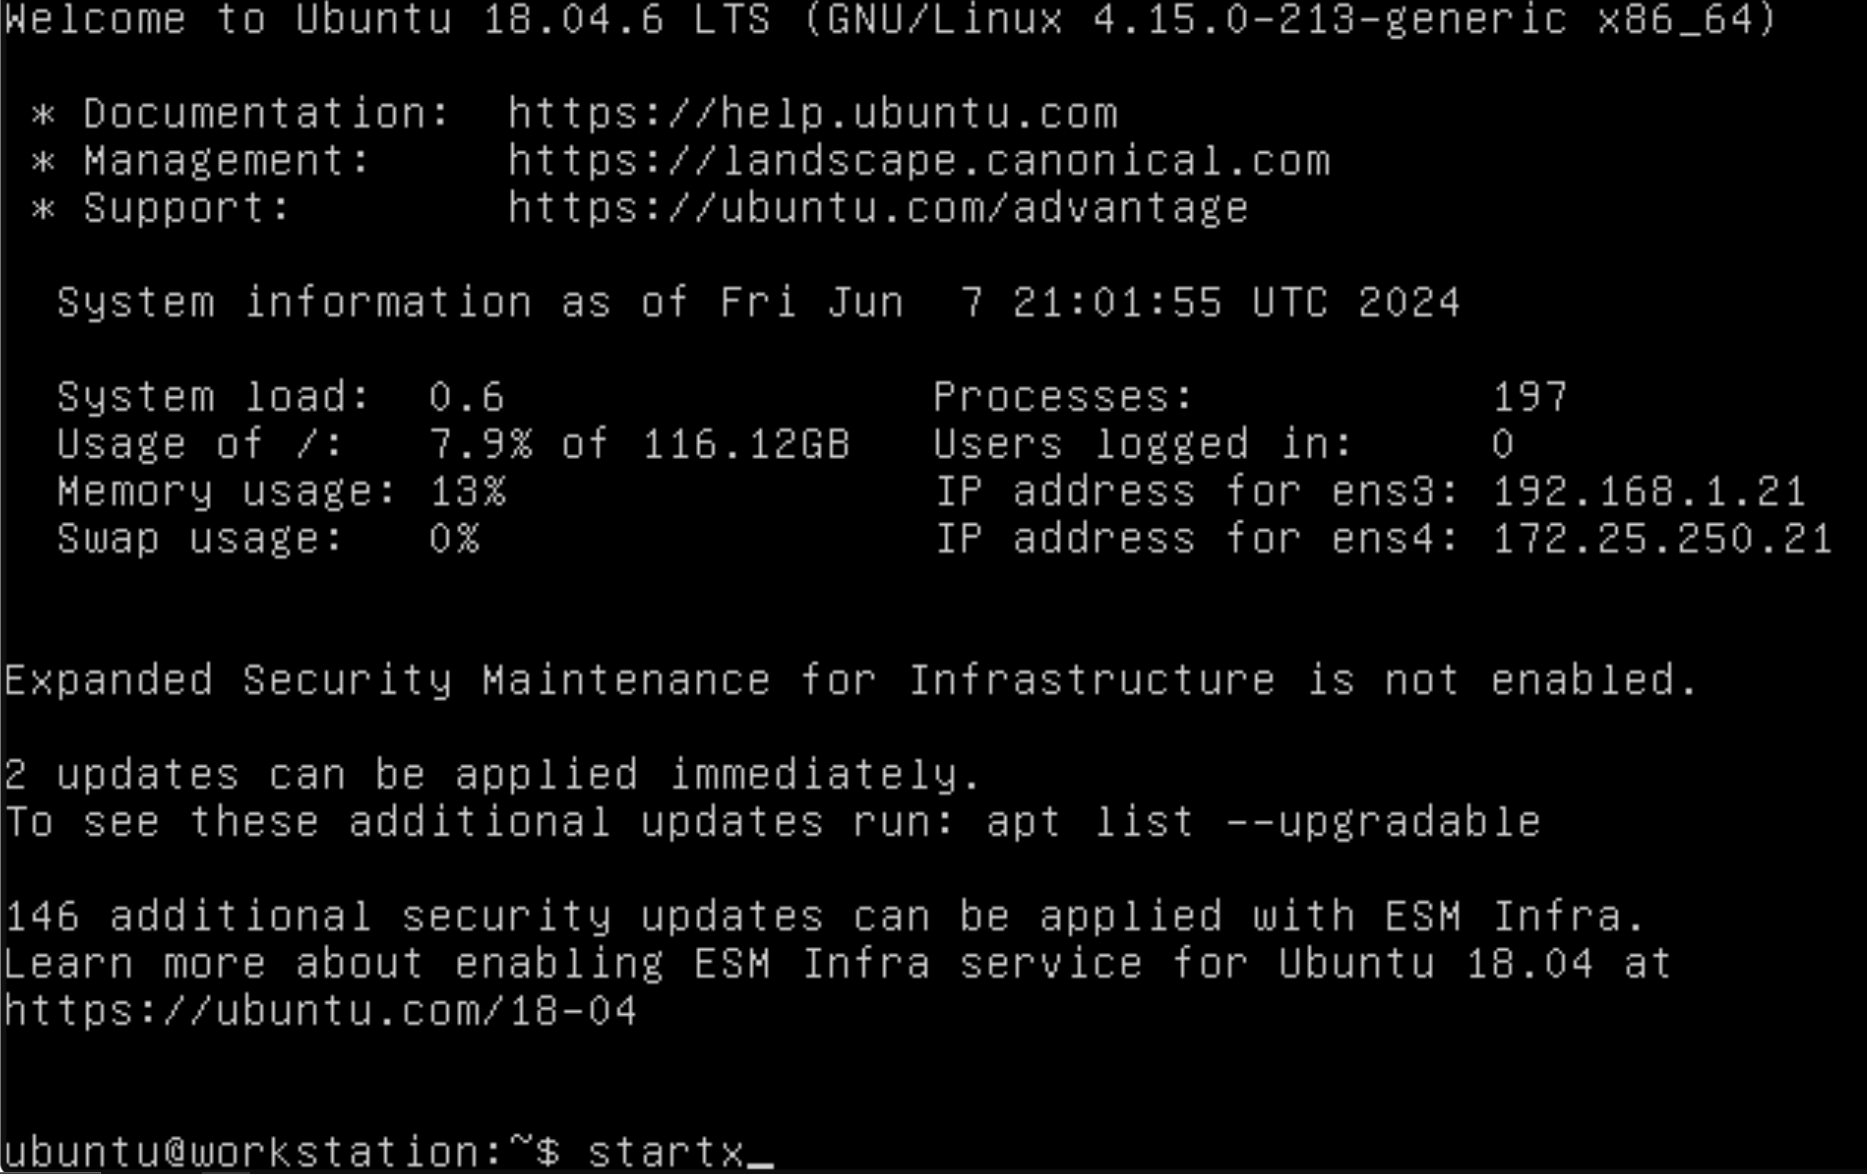
\includegraphics[width=\linewidth]{images/part1/step2.png}
        \end{center}
    \end{labstep}

    \begin{labstep}
        Open the web browser.
        Navigate to \textbf{192.168.1.20}, and log in to the dashboard as \textbf{admin} with the password \textbf{secret}.

        \begin{center}
            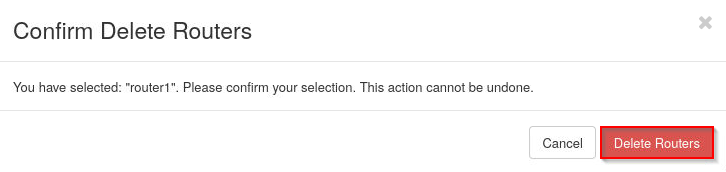
\includegraphics[scale=0.5]{images/part1/step3.png}
        \end{center}
    \end{labstep}

    \begin{labstep}
        Select the \textbf{demo} project.
        Navigate to \textbf{Network $>$ Security Groups} and click \textbf{Create Security Group}.

        \begin{center}
            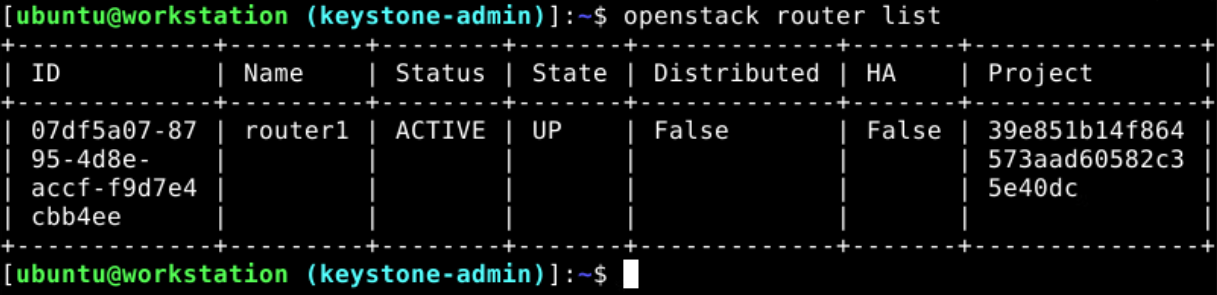
\includegraphics[width=\linewidth]{images/part1/step4.png}
        \end{center}
    \end{labstep}

    \begin{labstep}
        Enter \textbf{secgroup1} into the \textit{Name} field and click \textbf{Create Security Group}.

        \begin{center}
            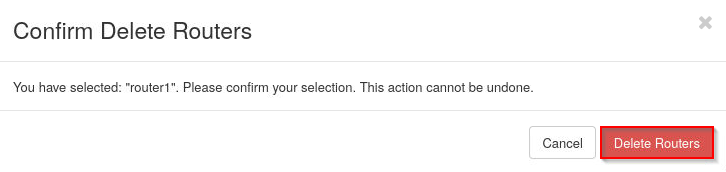
\includegraphics[width=\linewidth]{images/part1/step5.png}
        \end{center}
    \end{labstep}

    \begin{labstep}
        After creating the security group, you should be redirected to its rules page.
        If not, click \textbf{Manage Rules} in the same row as \textbf{secgroup1} on the \textbf{Security Groups} page to get there.
        From here, you can see that by default, the security group allows all egress (outgoing) traffic.
        No ingress rules are defined, so all incoming traffic is denied by default.
        Click \textbf{Add Rule} to add a new rule in the security group.

        \begin{center}
            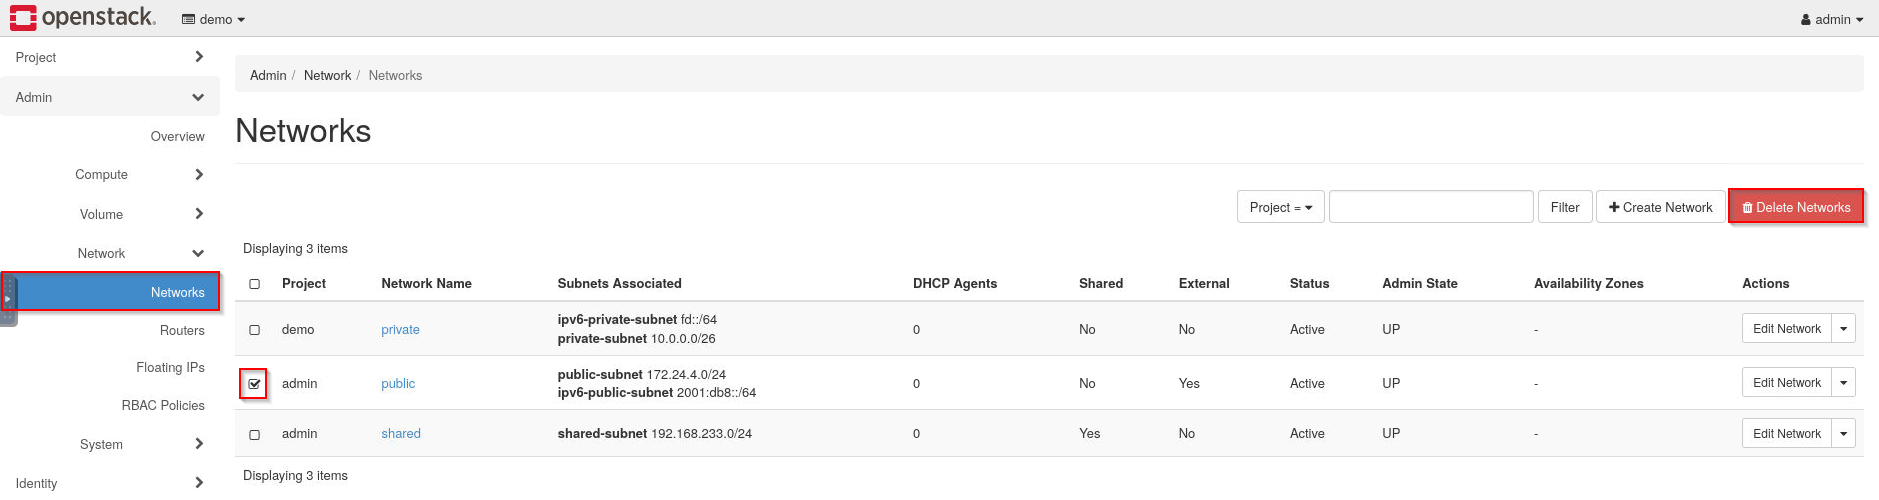
\includegraphics[width=\linewidth]{images/part1/step6.png}
        \end{center}
    \end{labstep}

    \begin{labstep}
        Select \textbf{All ICMP} from the \textit{Rule} dropdown and click \textbf{Add}.
        This allows ICMP traffic, including the \textbf{ping} command, to reach instances in this security group.

        \begin{center}
            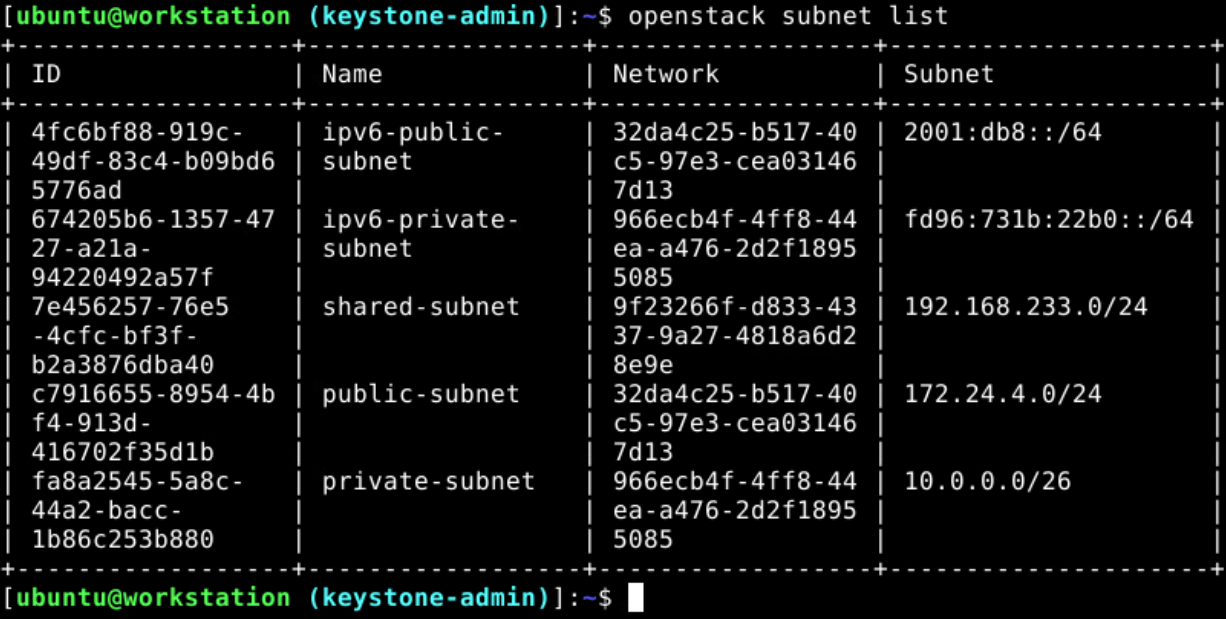
\includegraphics[width=\linewidth]{images/part1/step7.png}
        \end{center}
    \end{labstep}

    \begin{notebox}
        By default, \textit{Direction} is set to \textbf{Ingress} and \textit{CIDR} is set to \textbf{0.0.0.0/0}.
        \textbf{Ingress} specifies incoming traffic, and \textbf{0.0.0.0/0} specifies that the traffic is accepted from any IP address.
    \end{notebox}

    \begin{labstep}
        Click \textbf{Add Rule} again.

        \begin{center}
            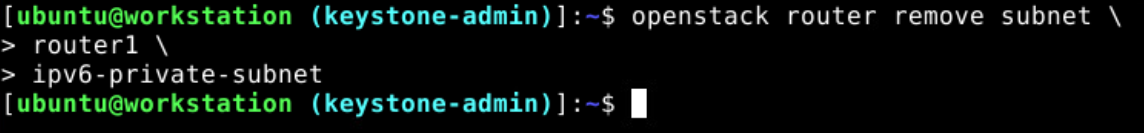
\includegraphics[width=\linewidth]{images/part1/step8.png}
        \end{center}
    \end{labstep}

    \begin{labstep}
        Now, we will create a rule to allow SSH ingress traffic.
        Since SSH works over TCP, leave \textit{Rule} as \textbf{Custom TCP Rule}.
        Under \textit{Port}, enter \textbf{22}, which is the default SSH port.
        Click \textbf{Add} to add the rule.

        \begin{center}
            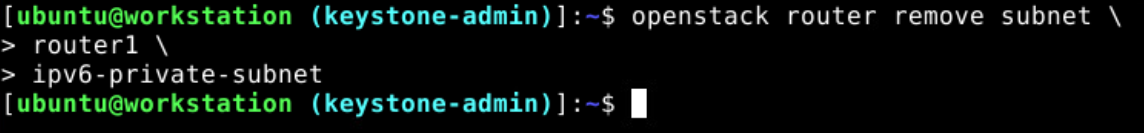
\includegraphics[width=\linewidth]{images/part1/step9.png}
        \end{center}
    \end{labstep}

    \begin{labstep}
        Log out of the \textit{Horizon Dashboard} and close the web browser.
    \end{labstep}

    \begin{labstep}
        If a terminal window is not already open, open one and source the \textbf{admin} credentials from the
        \textbf{\texttildemid/keystonerc-admin} file.
        \begin{lstlisting}
            ubuntu@workstation:~$ source ~/keystonerc-admin
        \end{lstlisting}

        \begin{center}
            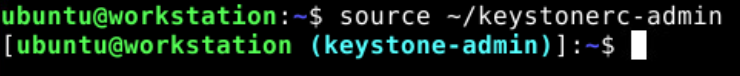
\includegraphics[width=\linewidth]{images/part1/step11.png}
        \end{center}
    \end{labstep}

    \begin{labstep}
        Before creating or modifying any security groups or rules, list the existing security groups to see what is already configured.
        \begin{lstlisting}
            [ubuntu@workstation (keystone-admin)]:~$ openstack security group list
        \end{lstlisting}

        \begin{center}
            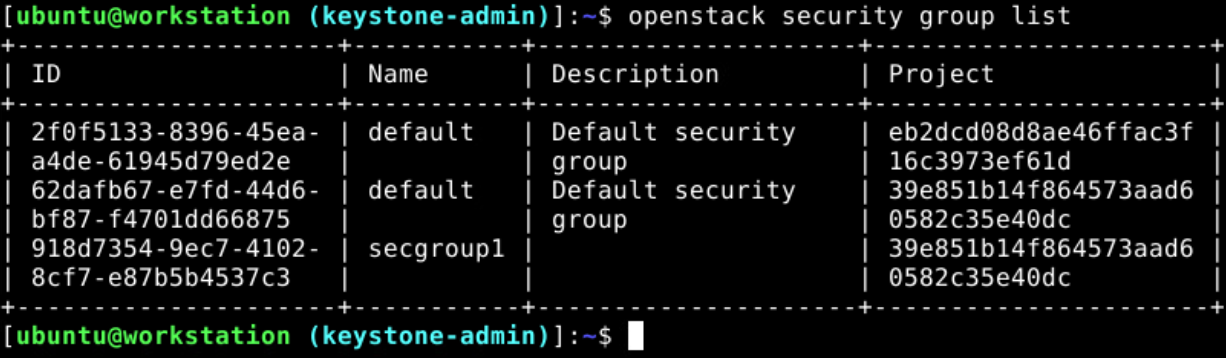
\includegraphics[width=\linewidth]{images/part1/step12.png}
        \end{center}
    \end{labstep}

    \begin{labstep}
        Now, we will recreate the \textbf{secgroup1} security group through the command line and add some additional rules necessary for connecting to an external instance.
        First, to demonstrate how to remove a rule from a security group, list the rules in the \textbf{secgroup1} security group and copy the ID of the ICMP rule.
        \begin{lstlisting}
            [ubuntu@workstation (keystone-admin)]:~$ openstack security group rule list \
            > secgroup1
        \end{lstlisting}

        \begin{center}
            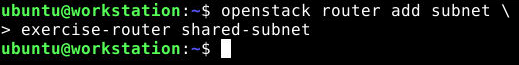
\includegraphics[width=\linewidth]{images/part1/step13.png}
        \end{center}
    \end{labstep}

    \begin{tipbox}
        Since we want to copy the ID value, we do not want the output to fit the width of the terminal window, which would wrap the ID across multiple lines and prevent copying.
        To prevent this, maximize the terminal window before running this command.
    \end{tipbox}
    \begin{tipbox}
        To copy a value from the terminal, select the desired string with the mouse, then either right-click and click \textbf{Copy} or press \textbf{Ctrl+Shift+C}.
    \end{tipbox}

    \begin{labstep}
        Use the ID for the ICMP rule to delete that rule.
        Note that you do not have to list \textbf{secgroup1} in this command because IDs in OpenStack are \textit{globally unique} within a deployment.
        \begin{lstlisting}
            [ubuntu@workstation (keystone-admin)]:~$ openstack security group rule delete \
            > 8b0035c8-f81e-451d-bf08-dd258ebca9f4
        \end{lstlisting}

        \begin{center}
            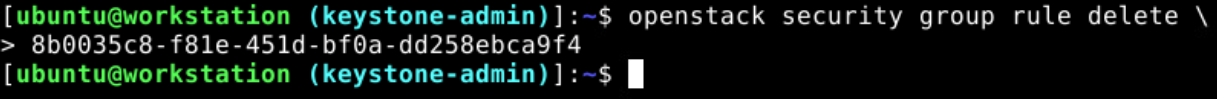
\includegraphics[width=\linewidth]{images/part1/step14.png}
        \end{center}
    \end{labstep}

    \begin{notebox}
        The actual ID value may differ.
    \end{notebox}
    \begin{tipbox}
        To paste a value to the command line, either right-click and click \textbf{Paste} or press \textbf{Ctrl+Shift+V}.
    \end{tipbox}

    \begin{labstep}
        List the rules in the \textbf{secgroup1} security group again to ensure the rule was deleted successfully.
        \begin{lstlisting}
            [ubuntu@workstation (keystone-admin)]:~$ openstack security group rule list \
            > secgroup1
        \end{lstlisting}

        \begin{center}
            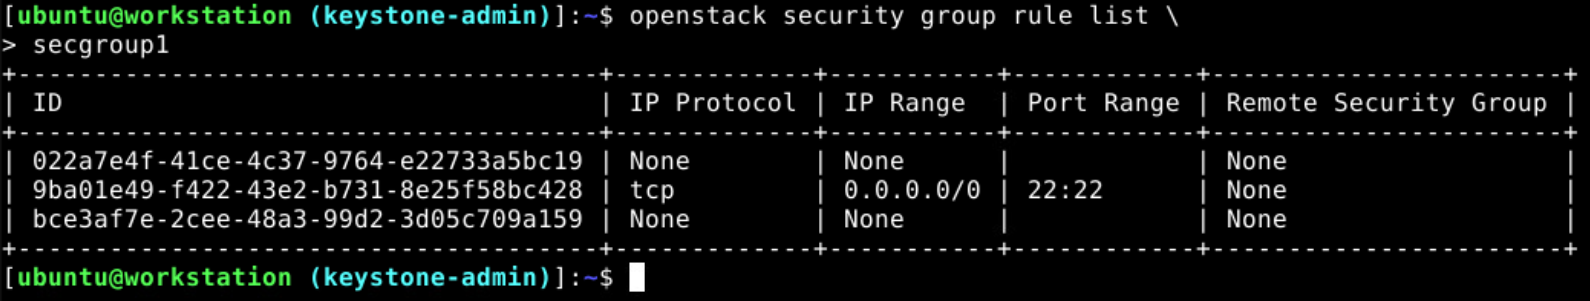
\includegraphics[width=\linewidth]{images/part1/step15.png}
        \end{center}
    \end{labstep}

    \begin{labstep}
        Delete the \textbf{secgroup1} security group.
        \begin{lstlisting}
            [ubuntu@workstation (keystone-admin)]:~$ openstack security group delete \
            > secgroup1
        \end{lstlisting}

        \begin{center}
            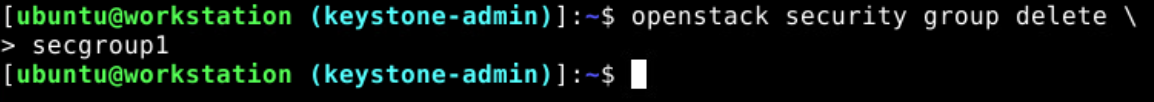
\includegraphics[width=\linewidth]{images/part1/step16.png}
        \end{center}
    \end{labstep}

    \begin{labstep}
        Create the \textbf{secgroup2} security group.
        \begin{lstlisting}
            [ubuntu@workstation (keystone-admin)]:~$ openstack security group create \
            > secgroup2
        \end{lstlisting}

        \begin{center}
            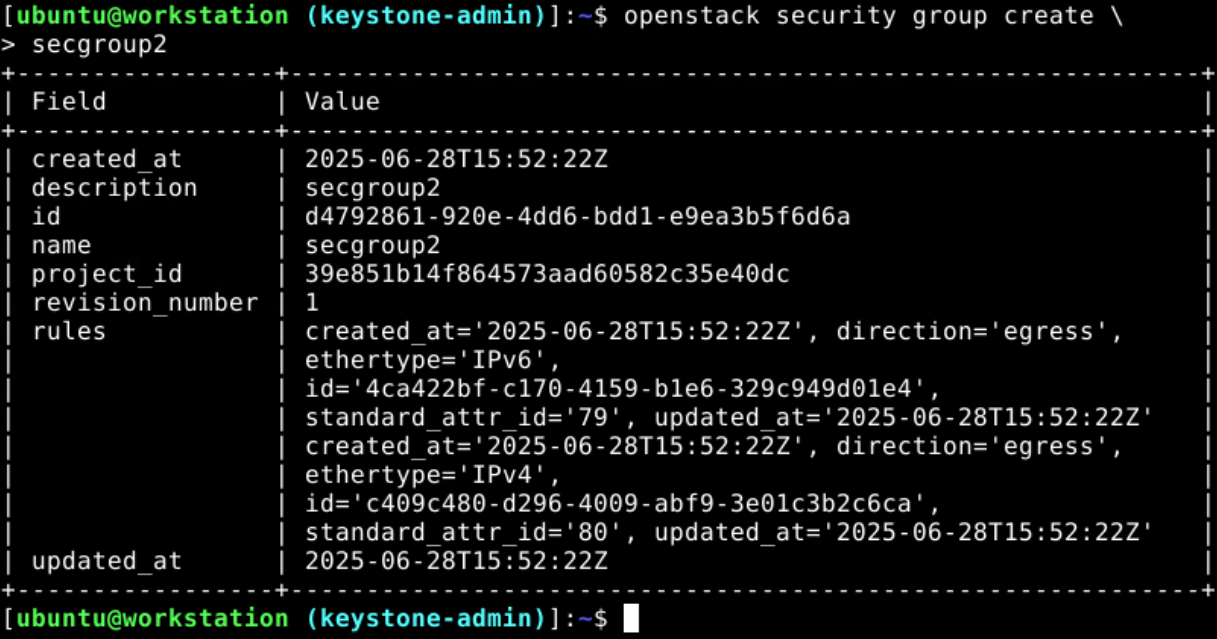
\includegraphics[width=\linewidth]{images/part1/step17.png}
        \end{center}
    \end{labstep}

    \begin{labstep}
        List the rules in the \textbf{secgroup2} security group.
        These are the default rules that exist upon creation.
        \begin{lstlisting}
            [ubuntu@workstation (keystone-admin)]:~$ openstack security group rule list \
            > secgroup2
        \end{lstlisting}

        \begin{center}
            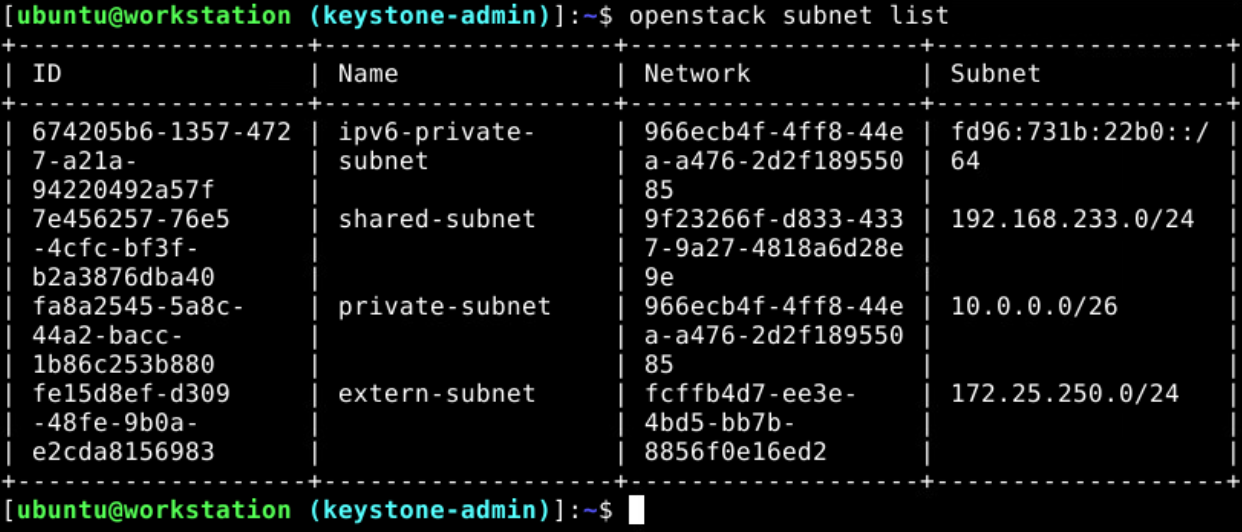
\includegraphics[width=\linewidth]{images/part1/step18.png}
        \end{center}
    \end{labstep}

    \begin{tipbox}
        You can use the command
        \begin{lstlisting}
            openstack security group rule show <rule_id>
        \end{lstlisting}
        to show the details of each rule and confirm that they are the same default rules you get when creating a security group through the Horizon Dashboard.
        The rules allow all outgoing traffic over IPv4 and IPv6.
    \end{tipbox}

    \begin{labstep}
        Add a security rule in the \textbf{secgroup2} security group to allow all incoming ICMP traffic.
        \begin{lstlisting}
            [ubuntu@workstation (keystone-admin)]:~$ openstack security group rule create \
            > --protocol icmp \
            > secgroup2
        \end{lstlisting}

        \begin{center}
            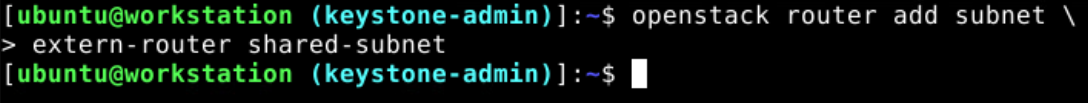
\includegraphics[width=\linewidth]{images/part1/step19.png}
        \end{center}
    \end{labstep}

    \begin{notebox}
        If no additional arguments are given, the direction defaults to \textbf{ingress} and the remote IP defaults to \textbf{0.0.0.0/0}.
        In other words, it allows all incoming traffic over the given protocol.
    \end{notebox}

    \begin{labstep}
        List the rules in the \textbf{secgroup2} security group again to ensure the ICMP rule was created successfully.
        \begin{lstlisting}
            [ubuntu@workstation (keystone-admin)]:~$ openstack security group rule list \
            > secgroup2
        \end{lstlisting}

        \begin{center}
            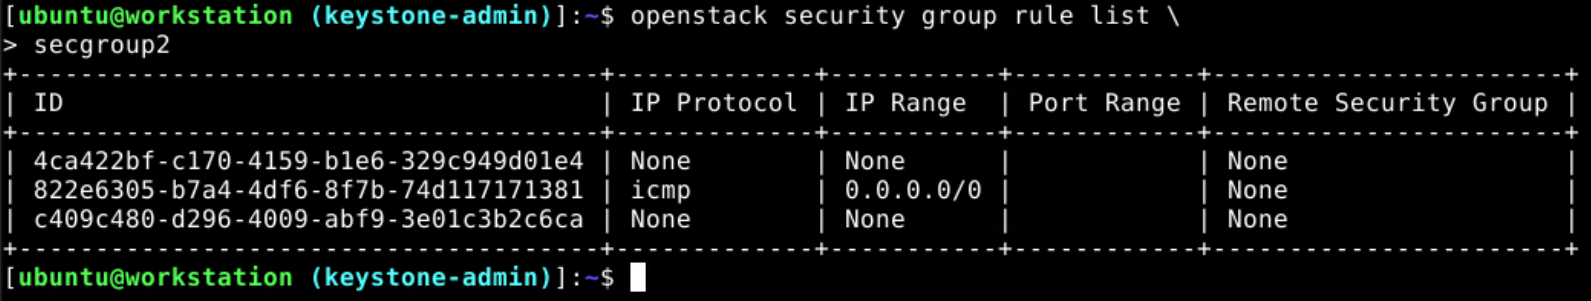
\includegraphics[width=\linewidth]{images/part1/step20.png}
        \end{center}
    \end{labstep}

    \begin{labstep}
        Add another security rule to allow remote connection using SSH on the default port 22.
        \begin{lstlisting}
            [ubuntu@workstation (keystone-admin)]:~$ openstack security group rule create \
            > --protocol tcp \
            > --dst-port 22 \
            > secgroup2
        \end{lstlisting}

        \begin{center}
            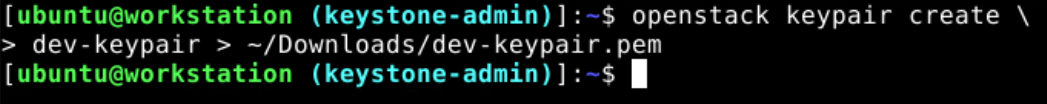
\includegraphics[width=\linewidth]{images/part1/step21.png}
        \end{center}
    \end{labstep}

    \begin{labstep}
        List the rules in the \textbf{secgroup2} security group again to ensure the SSH rule was created successfully.
        \begin{lstlisting}
            [ubuntu@workstation (keystone-admin)]:~$ openstack security group rule list \
            > secgroup2
        \end{lstlisting}

        \begin{center}
            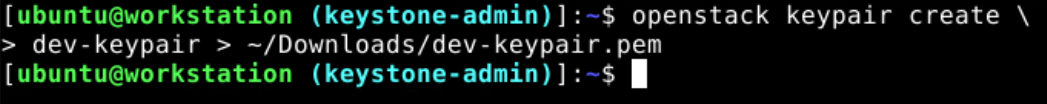
\includegraphics[width=\linewidth]{images/part1/step22.png}
        \end{center}
    \end{labstep}

    \begin{labstep}
        Leave the terminal window open and continue to the next task.
    \end{labstep}

\end{enumerate}

%%%%%%%%%%%
% Section 2
%%%%%%%%%%%
\section{Applying Security Groups to Instances}\label{sec:applying-security-groups-to-instances}
In order for a security group's rules to apply to instance, the security group must be applied to one of the instance's interfaces.
In these labs, instances will only have one interface, so a security group can be thought of as applying to the whole instance.
Additionally, an interface may have more than one security group applied.
Security groups can be added to an instance when the instance is created, and they can be added, removed, or modified at any time.
This section will walk through adding and removing an instance's security groups with both the \textit{OpenStack Unified CLI} and the \textit{Horizon Dashboard}.

\begin{enumerate}
    \begin{labstep}
        If a terminal window is not already open, open one and source the admin credentials from the \textbf{\texttildemid/keystonerc-admin} file.
        \begin{lstlisting}
            ubuntu@workstation:~$ source ~/keystonerc-admin
        \end{lstlisting}

        \begin{center}
            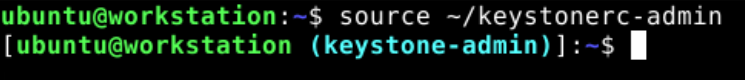
\includegraphics[width=\linewidth]{images/part2/step1.png}
        \end{center}
    \end{labstep}

    \begin{labstep}
        A security group can be applied to an instance at creation from the command line.
        Create an instance with the security group \textbf{secgroup2} applied to it.
        \begin{lstlisting}
            [ubuntu@workstation (keystone-admin)]:~$ openstack server create \
            > --image ubuntu \
            > --flavor m1.small \
            > --network shared \
            > --security-group secgroup2 \
            > instance1
        \end{lstlisting}

        \begin{center}
            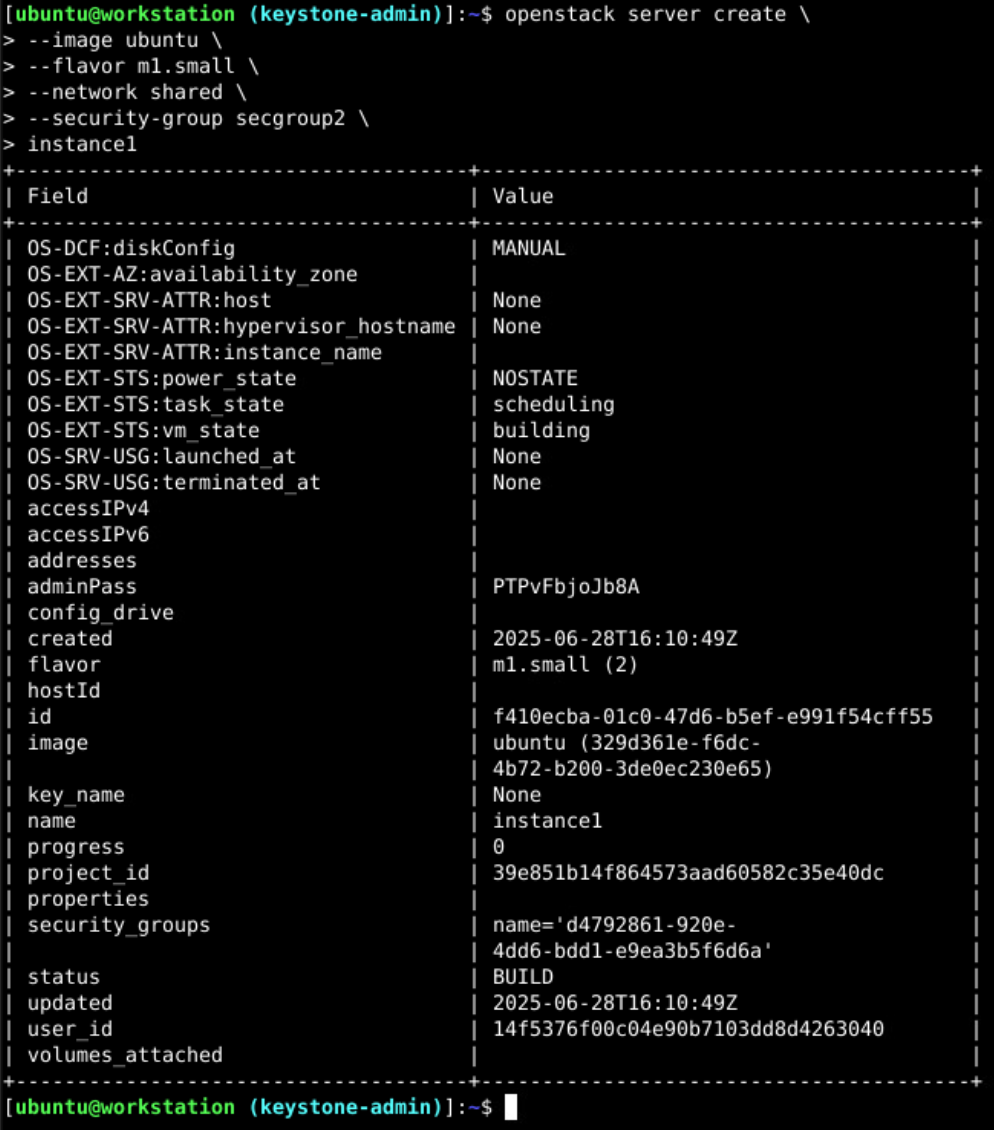
\includegraphics[width=\linewidth]{images/part2/step2.png}
        \end{center}
    \end{labstep}

    \begin{labstep}
        The output of the previous step should have shown the ID of \textbf{secgroup2} in the \textbf{security\_groups} row.
        To get a result that easier to understand and verify that \textbf{secgroup2} is attached to the instance, we can show the details of the instance with a couple extra arguments.
        \begin{lstlisting}
            [ubuntu@workstation (keystone-admin)]:~$ openstack server show \
            > -c security_groups \
            > instance1
        \end{lstlisting}

        \begin{center}
            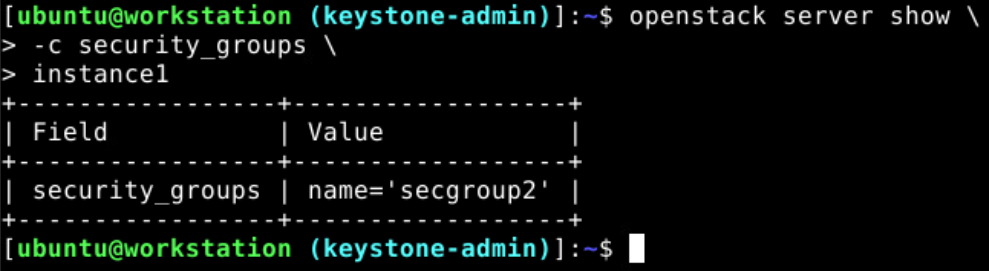
\includegraphics[width=\linewidth]{images/part2/step3.png}
        \end{center}
    \end{labstep}

    \begin{tipbox}
        The \textbf{-c security\_groups} argument specifies that we want only the \textbf{security\_groups} row in the output.
    \end{tipbox}

    \begin{labstep}
        Remove \textbf{secgroup2} from the instance.
        \begin{lstlisting}
            [ubuntu@workstation (keystone-admin)]:~$ openstack server remove security group \
            > instance1 secgroup2
        \end{lstlisting}

        \begin{center}
            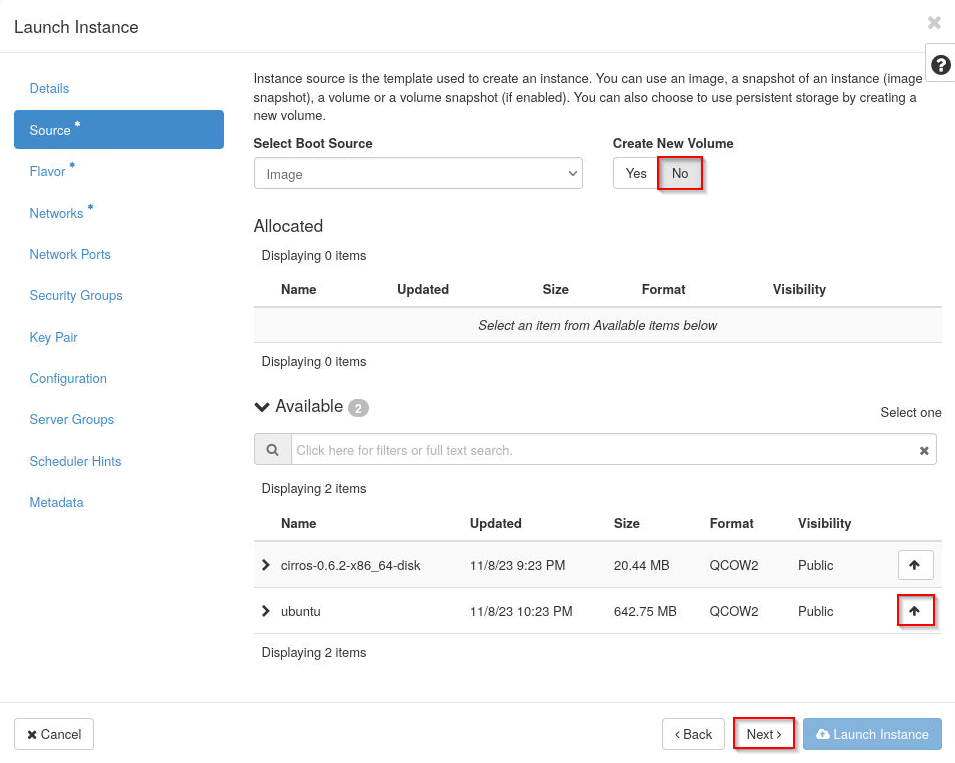
\includegraphics[width=\linewidth]{images/part2/step4.png}
        \end{center}
    \end{labstep}

    \begin{notebox}
        This command may echo the string \textbf{keys: ['name']}.
        Ignore this output; the command still works as intended.
    \end{notebox}

    \begin{labstep}
        Verify that the security group is no longer applied to the instance.
        You should receive an error message saying the column name is not recognized.
        \begin{lstlisting}
            [ubuntu@workstation (keystone-admin)]:~$ openstack server show \
            > -c security_groups \
            > instance1
        \end{lstlisting}

        \begin{center}
            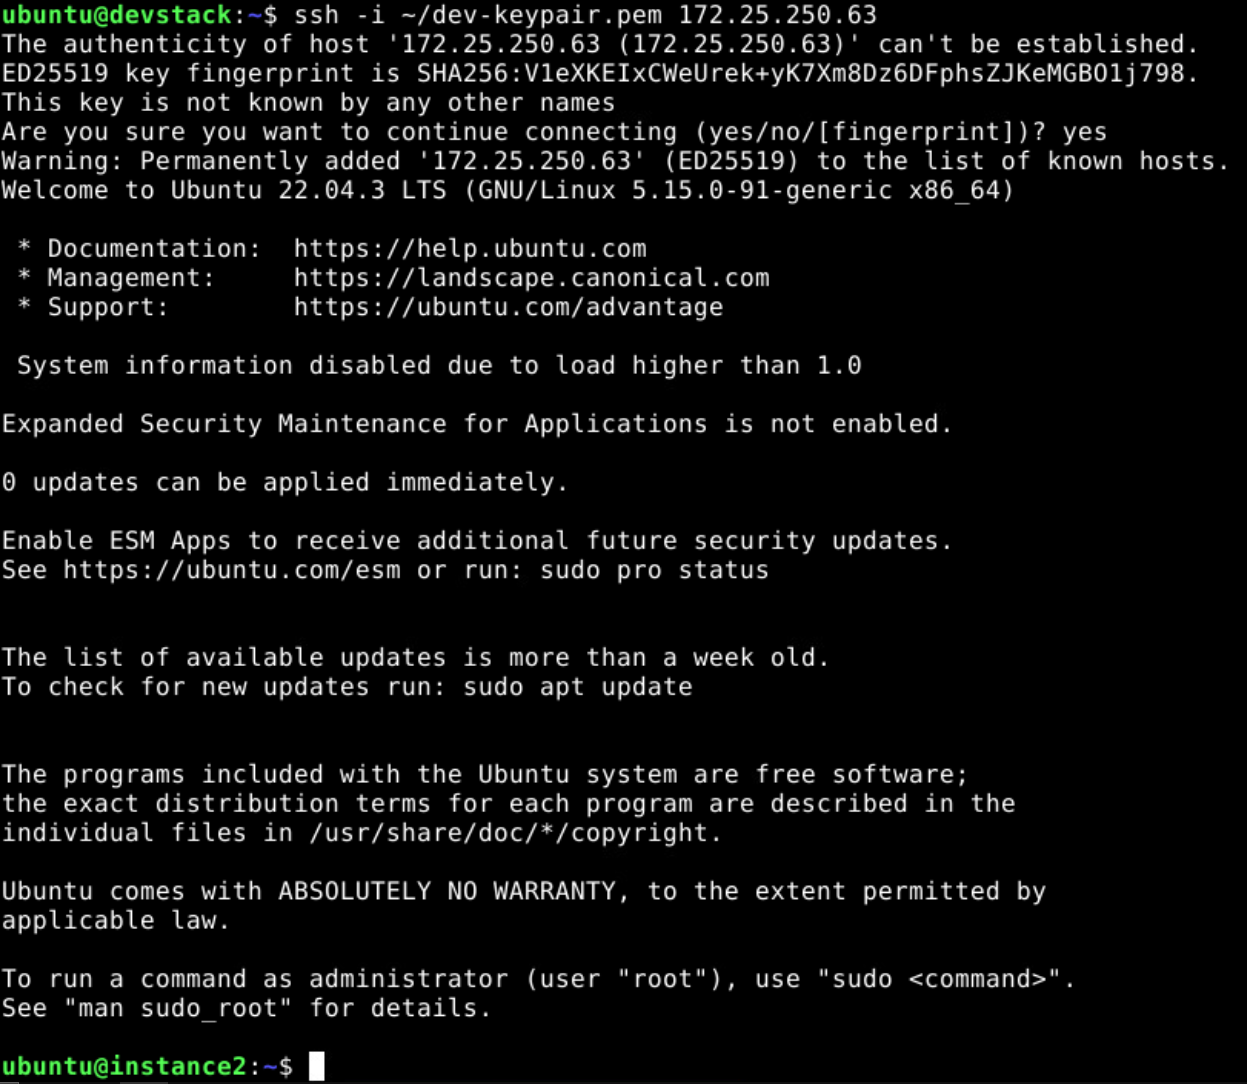
\includegraphics[width=\linewidth]{images/part2/step5.png}
        \end{center}
    \end{labstep}

    \begin{labstep}
        A security group can also be added to an instance after the instance is created.
        Add \textbf{secgroup2} back to the instance.
        \begin{lstlisting}
            [ubuntu@workstation (keystone-admin)]:~$ openstack server add security group \
            > instance1 secgroup2
        \end{lstlisting}

        \begin{center}
            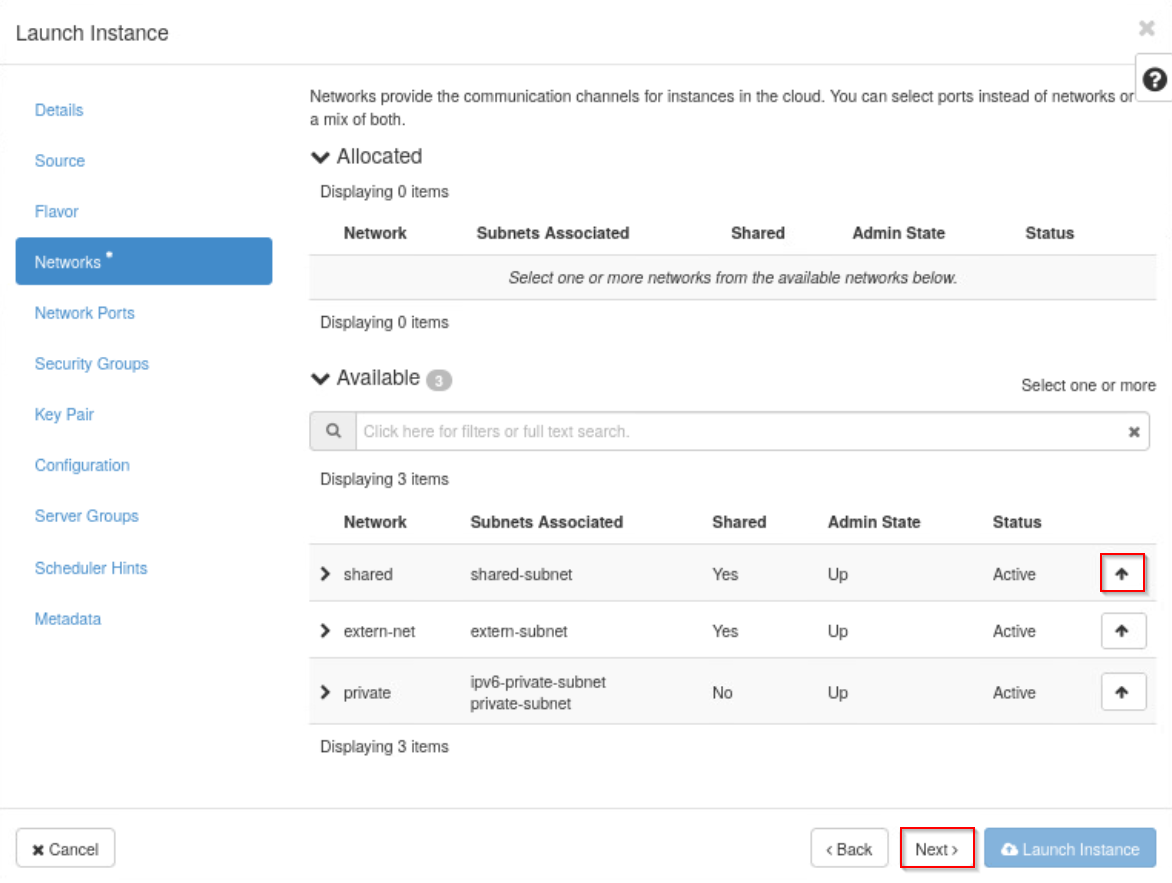
\includegraphics[width=\linewidth]{images/part2/step6.png}
        \end{center}
    \end{labstep}

    \begin{notebox}
        This command may echo the string \textbf{keys: ['name']}.
        Ignore this output; the command still works as intended.
    \end{notebox}

    \begin{labstep}
        Verify that the security group is once again applied to the instance.
        \begin{lstlisting}
            [ubuntu@workstation (keystone-admin)]:~$ openstack server show \
            > -c security_groups \
            > instance1
        \end{lstlisting}

        \begin{center}
            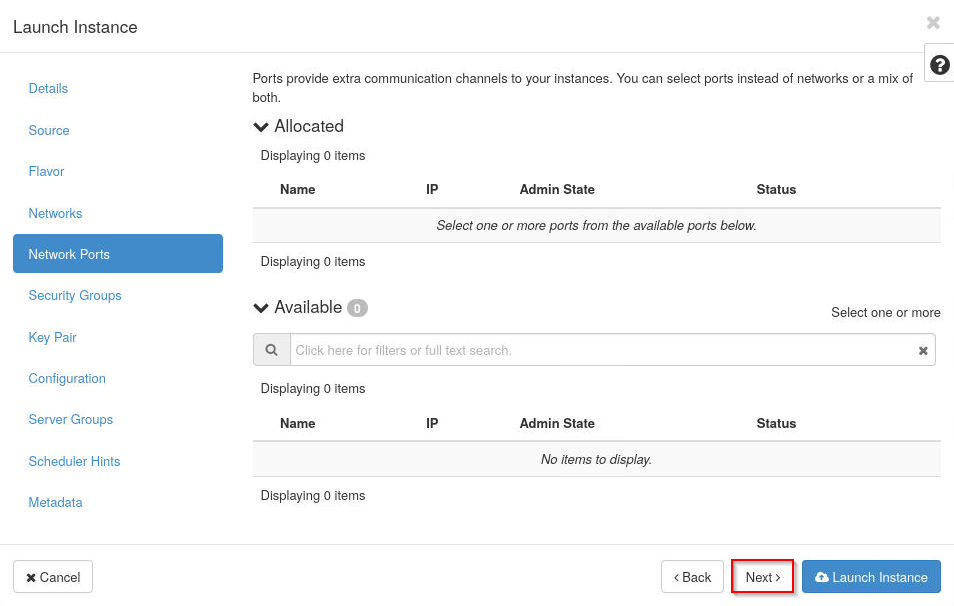
\includegraphics[width=\linewidth]{images/part2/step7.png}
        \end{center}
    \end{labstep}

    \begin{labstep}
        Delete \textbf{instance1}.
        We will recreate it from the Horizon Dashboard to demonstrate adding a security group to an instance at creation time from the dashboard.
        \begin{lstlisting}
            [ubuntu@workstation (keystone-admin)]:~$ openstack server delete instance1
        \end{lstlisting}

        \begin{center}
            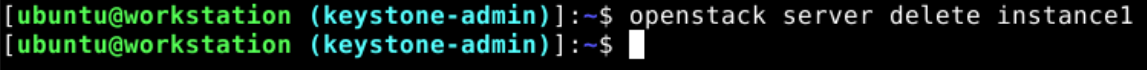
\includegraphics[width=\linewidth]{images/part2/step8.png}
        \end{center}
    \end{labstep}

    \begin{labstep}
        Leave the terminal window open, and open the web browser.
        Navigate to \textbf{192.168.1.20}, and log in to the dashboard as \textbf{admin} with the password \textbf{secret}.

        \begin{center}
            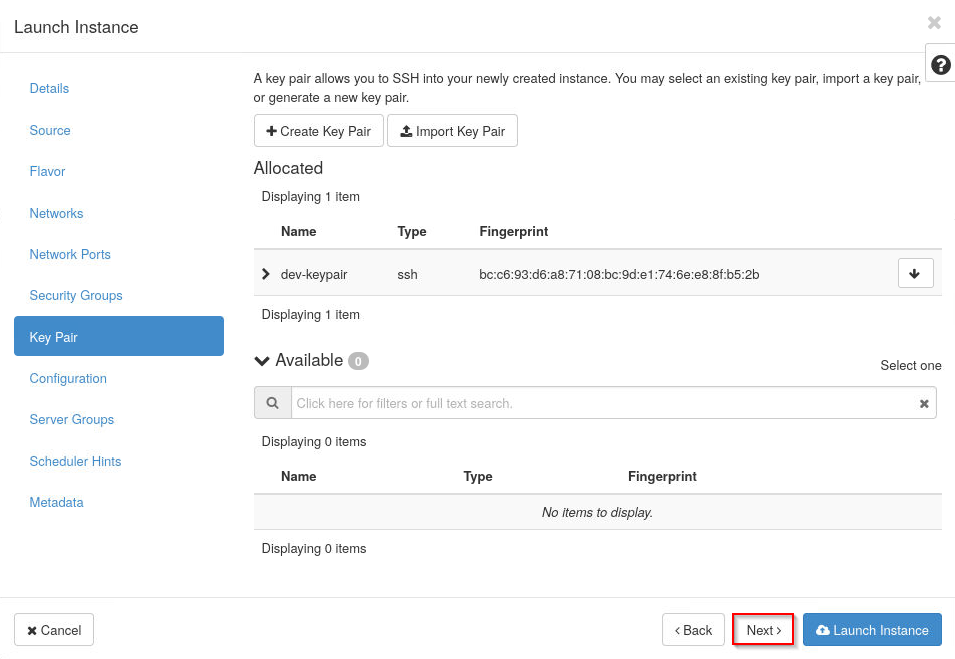
\includegraphics[scale=0.5]{images/part2/step9.png}
        \end{center}
    \end{labstep}

    \begin{labstep}
        Select the \textbf{demo} project.
        Navigate to \textbf{Project $>$ Compute $>$ Instances}, and click \textbf{Launch Instance}.

        \begin{center}
            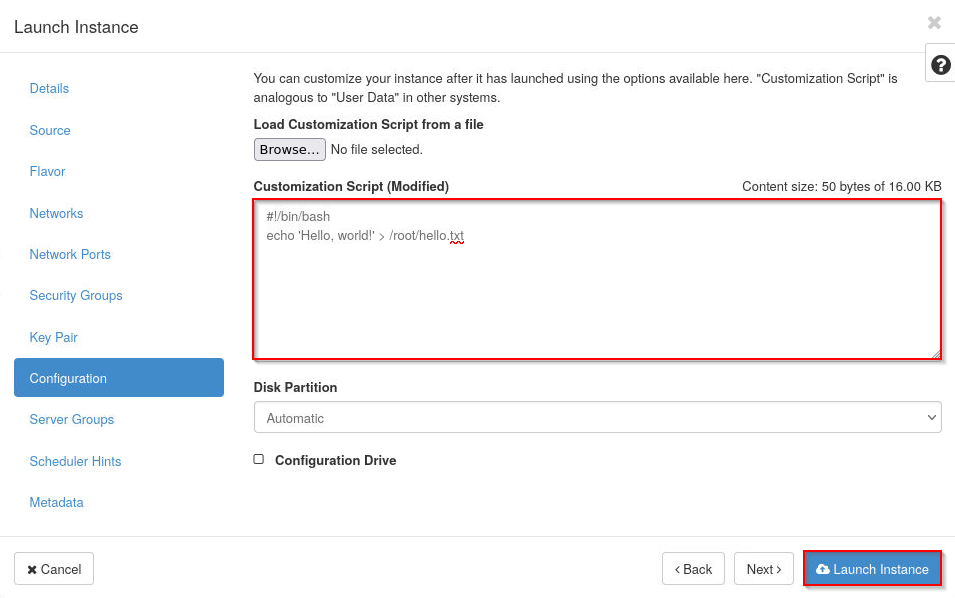
\includegraphics[width=\linewidth]{images/part2/step10.png}
        \end{center}
    \end{labstep}

    \begin{labstep}
        In the \textit{Details} tab, type \textbf{instance1} in the \textit{Instance Name} field.
        Click \textbf{Next}.

        \begin{center}
            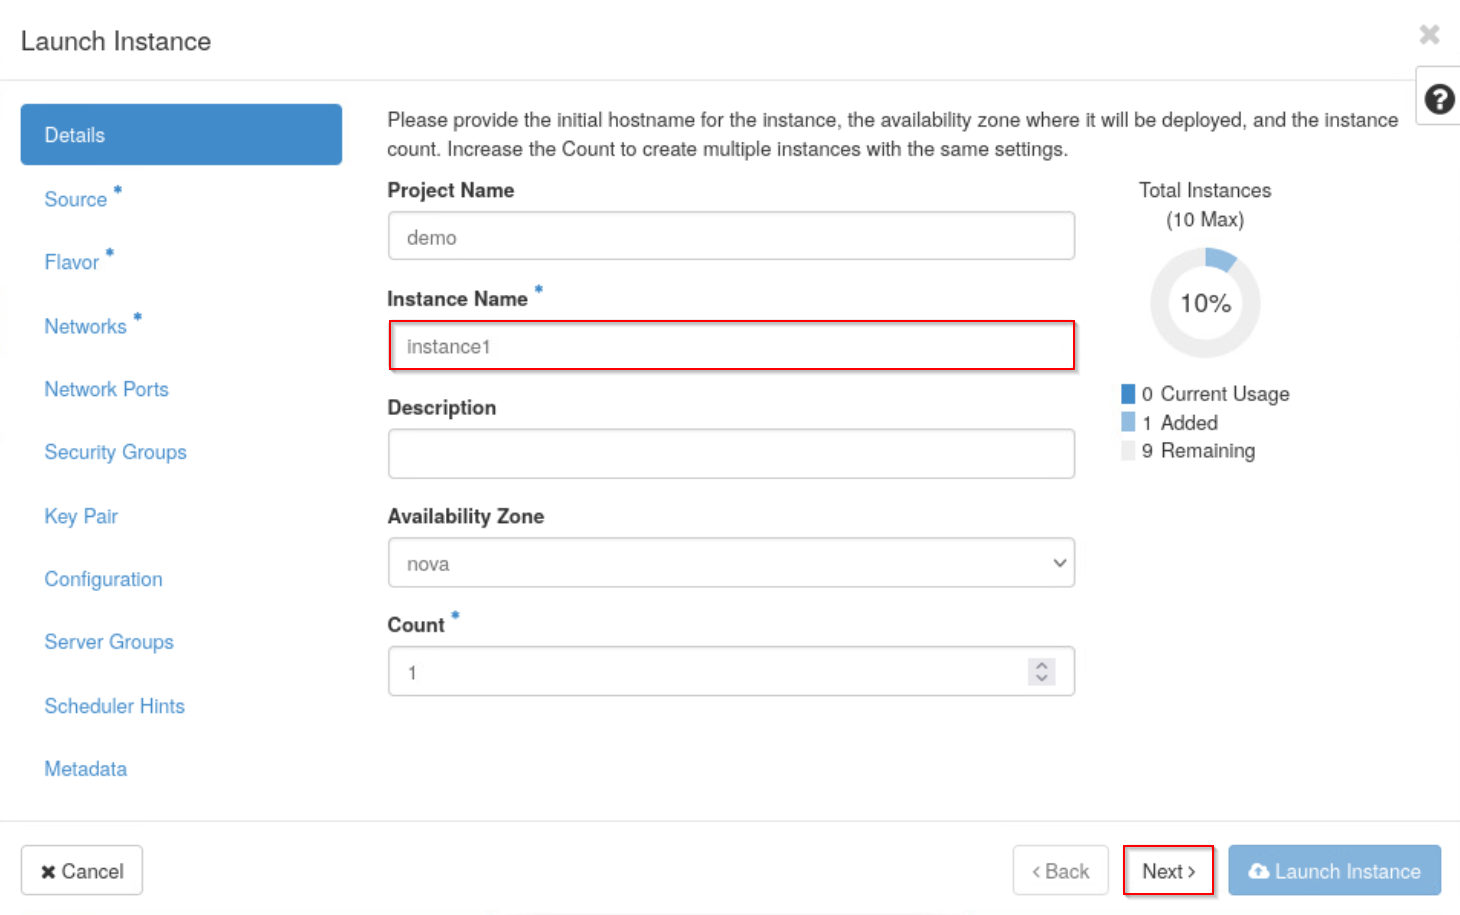
\includegraphics[width=\linewidth]{images/part2/step11.png}
        \end{center}
    \end{labstep}

    \begin{labstep}
        In the \textit{Source} tab, set \textit{Create New Volume} to \textbf{No}, and scroll down (if needed) to select the \textbf{ubuntu} image.
        Click \textbf{Next}.

        \begin{center}
            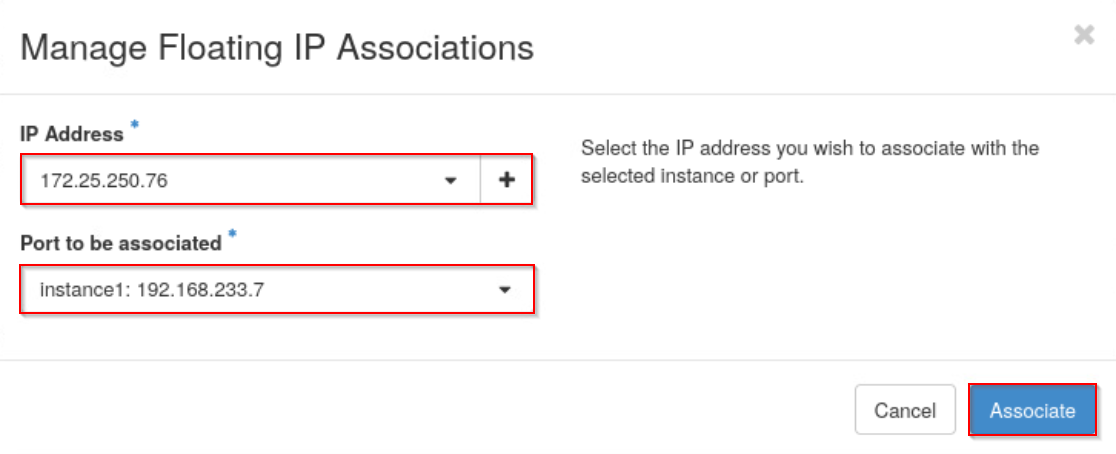
\includegraphics[width=\linewidth]{images/part2/step12.png}
        \end{center}
    \end{labstep}

    \begin{stopbox}
        Before proceeding to the next step, confirm that \textbf{ubuntu} appears in the \textit{Allocated} section.
    \end{stopbox}

    \begin{labstep}
        In the \textit{Flavor} tab, scroll down (if needed) to select the \textbf{m1.small} flavor.
        Click \textbf{Next}.

        \begin{center}
            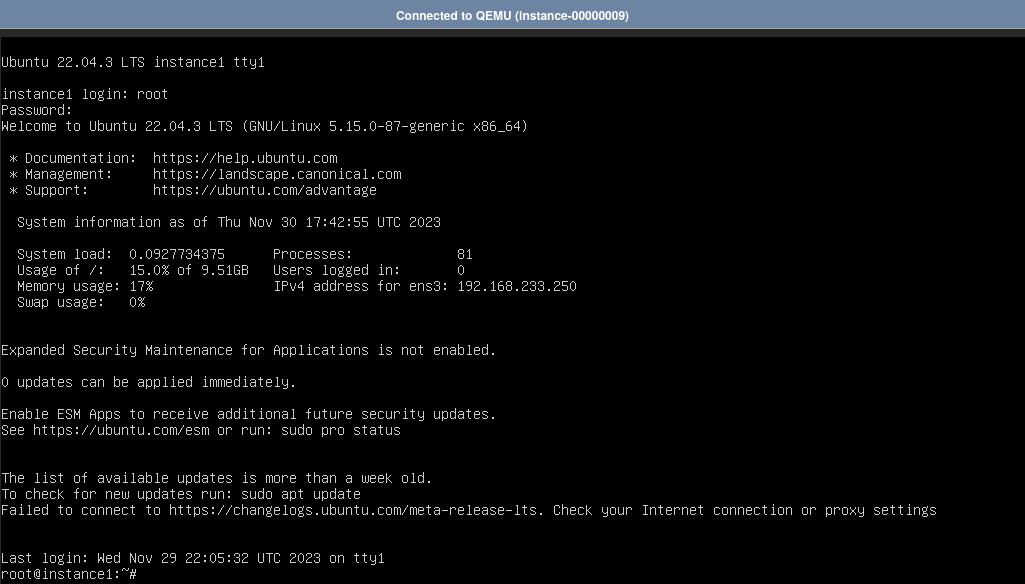
\includegraphics[width=\linewidth]{images/part2/step13.png}
        \end{center}
    \end{labstep}

    \begin{stopbox}
        Before proceeding to the next step, confirm that \textbf{m1.small} appears in the \textit{Allocated} section.
    \end{stopbox}

    \begin{labstep}
        In the \textit{Networks} tab, select the \textbf{shared} network.
        Navigate to the \textbf{Security Groups} tab.

        \begin{center}
            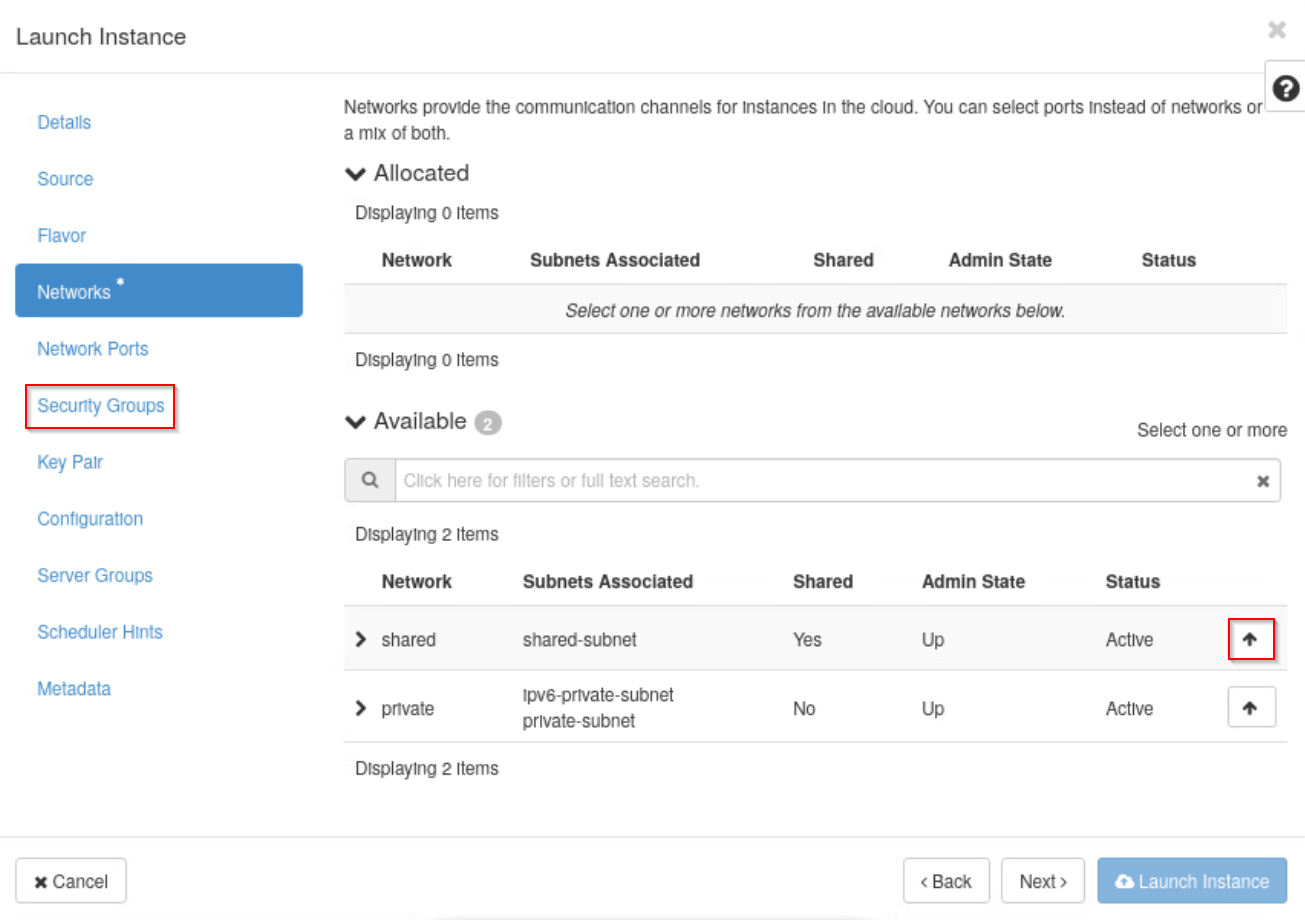
\includegraphics[width=\linewidth]{images/part2/step14.png}
        \end{center}
    \end{labstep}

    \begin{stopbox}
        Before proceeding to the next step, confirm that \textbf{shared} appears in the \textit{Allocated} section.
    \end{stopbox}

    \begin{labstep}
        In the \textit{Security Groups} tab, deselect the \textbf{default} security group since we have our own to apply.
        Scroll down (if needed) to select the \textbf{secgroup2} security group.
        This will apply the security group to all interfaces on the instance.
        Click \textbf{Launch Instance}.

        \begin{center}
            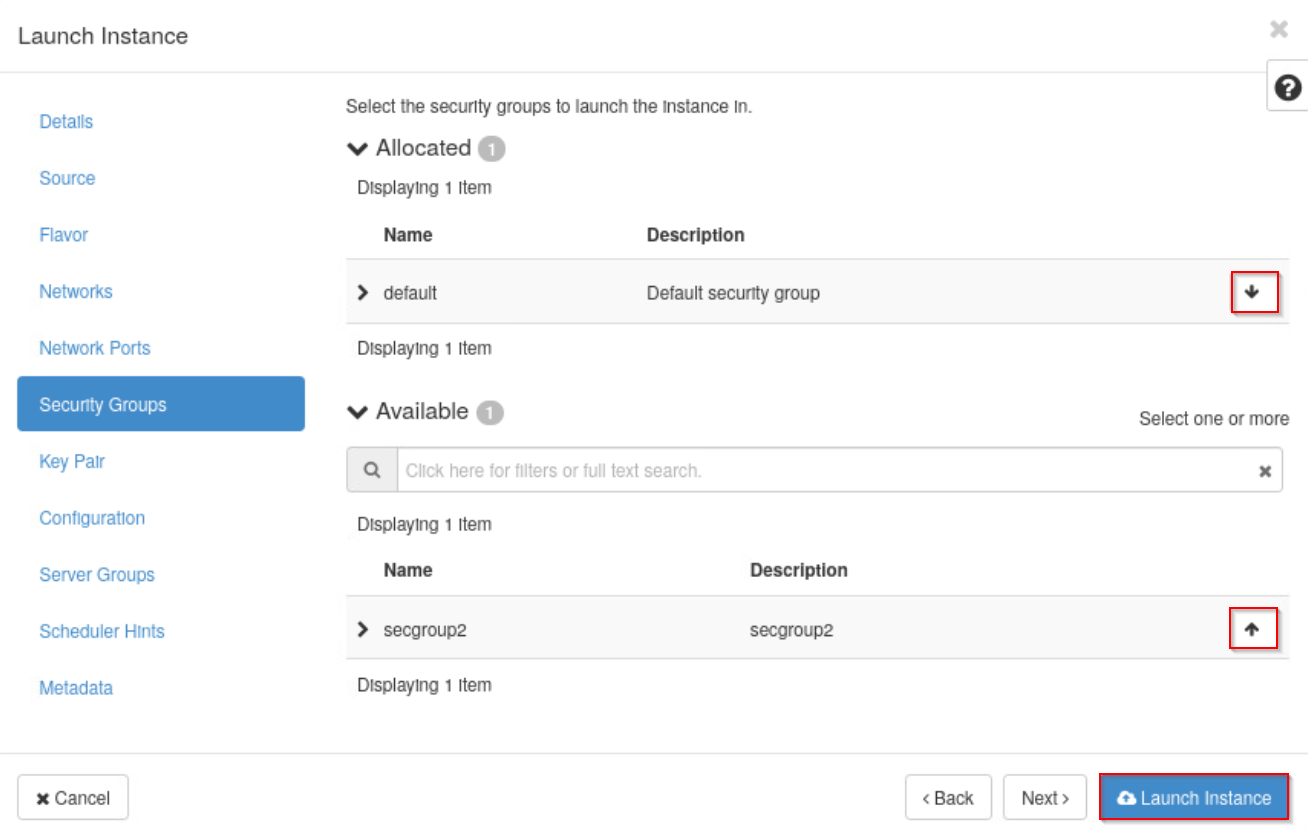
\includegraphics[width=\linewidth]{images/part2/step15.png}
        \end{center}
    \end{labstep}

    \begin{stopbox}
        Before proceeding to the next step, confirm that \textbf{secgroup2} appears in the \textit{Allocated} section.
    \end{stopbox}

    \begin{labstep}
        You should be redirected to the \textbf{Project $>$ Compute $>$ Instances} page.
        The security groups and rules applied to an instance can be found by clicking the instance's name.

        \begin{center}
            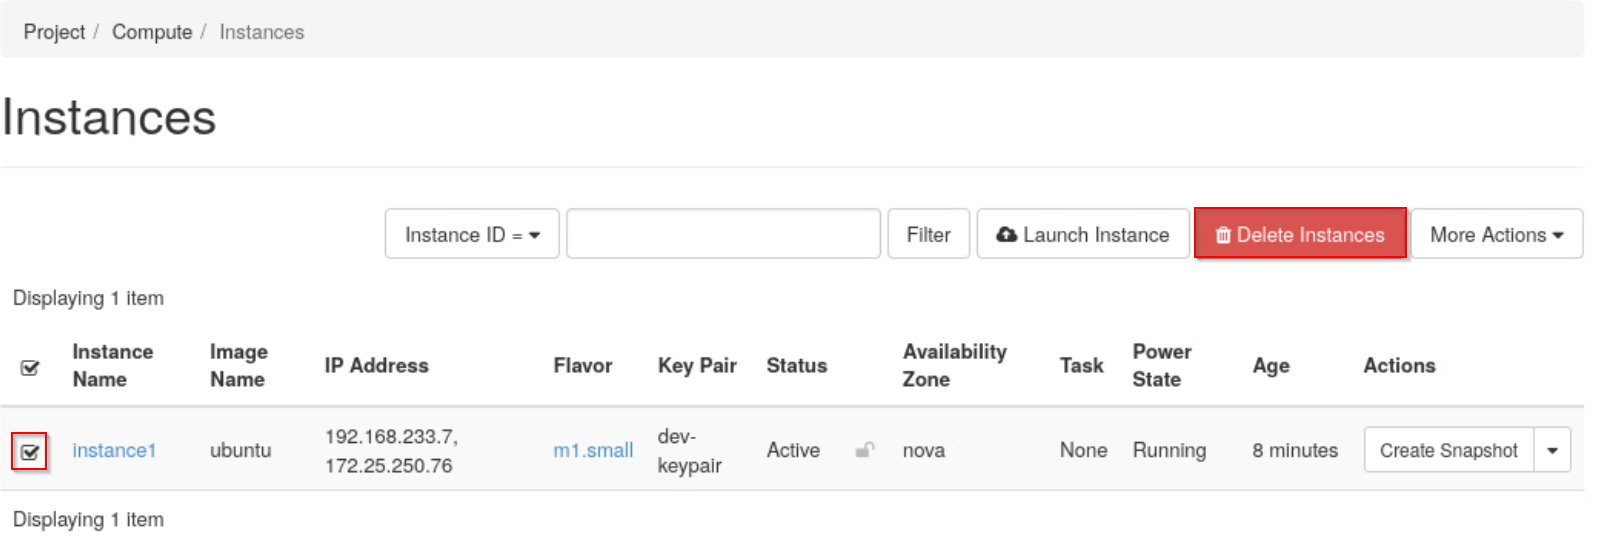
\includegraphics[width=\linewidth]{images/part2/step16.png}
        \end{center}
    \end{labstep}

    \begin{labstep}
        On the \textit{Overview} tab of the \textit{instance1} page, scroll down to view the \textit{Security Groups} section.
        In this case, you should see that \textbf{secgroup2} allows all IPv4 and IPv6 egress traffic by default, and you should see the two rules we added for ICMP and SSH (TCP port 22).

        \begin{center}
            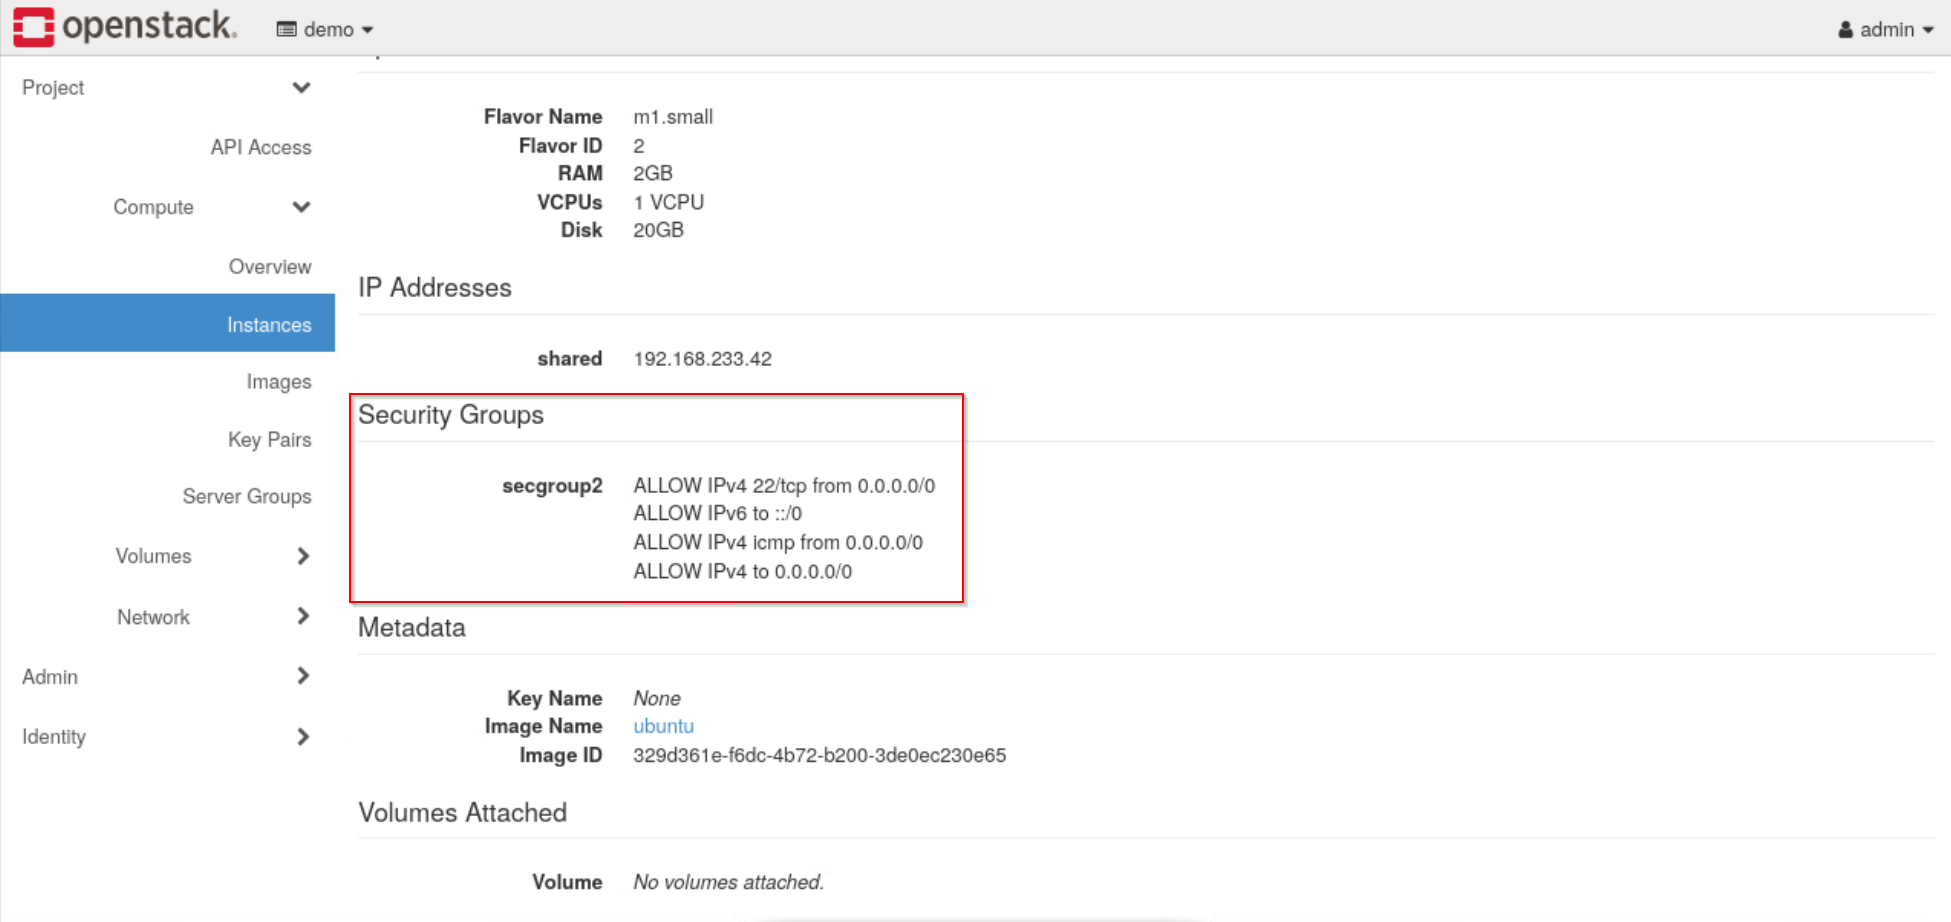
\includegraphics[width=\linewidth]{images/part2/step17.png}
        \end{center}
    \end{labstep}

    \begin{notebox}
        If no security group is applied to an instance, the \textit{Security Groups} section will simply say ``Not available''.
    \end{notebox}

    \begin{labstep}\label{it:secgroup}
        Navigate back to \textbf{Project $>$ Compute $>$ Instances}.
        To view and edit the security groups of an instance from the dashboard, click the dropdown next to \textbf{Create Snapshot}, and click \textbf{Edit Security Groups}.

        \begin{center}
            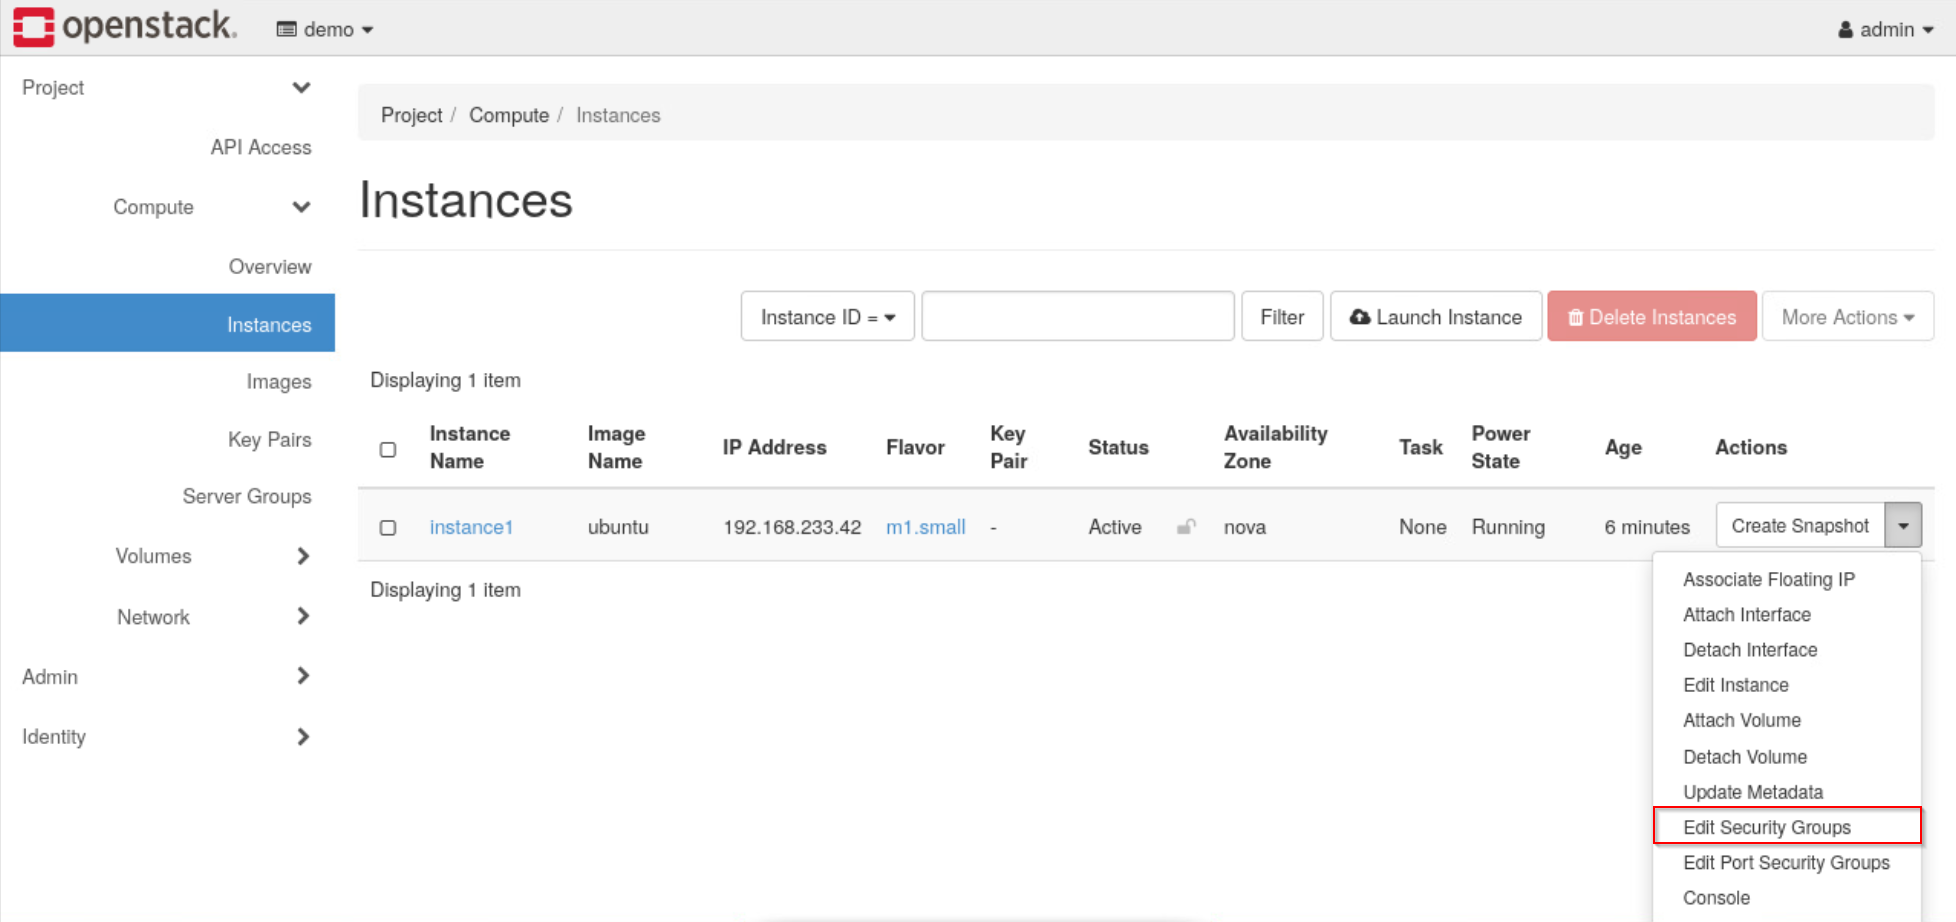
\includegraphics[width=\linewidth]{images/part2/step18.png}
        \end{center}
    \end{labstep}

    \begin{notebox}
        This option will edit security groups for all interfaces on the instance.
        Notice that there is also an option to \textbf{Edit Port Security Groups}, which allows you to edit security groups for individual interfaces on the instance.
    \end{notebox}

    \begin{labstep}
        In the \textbf{Edit Instance} popup, the \textbf{Instance Security Groups} list contains the security groups that are currently applied to the instance.
        Remove \textbf{secgroup2} from this instance by clicking the \textbf{-} button next to that group, and click \textbf{Save} to finalize the change.

        \begin{center}
            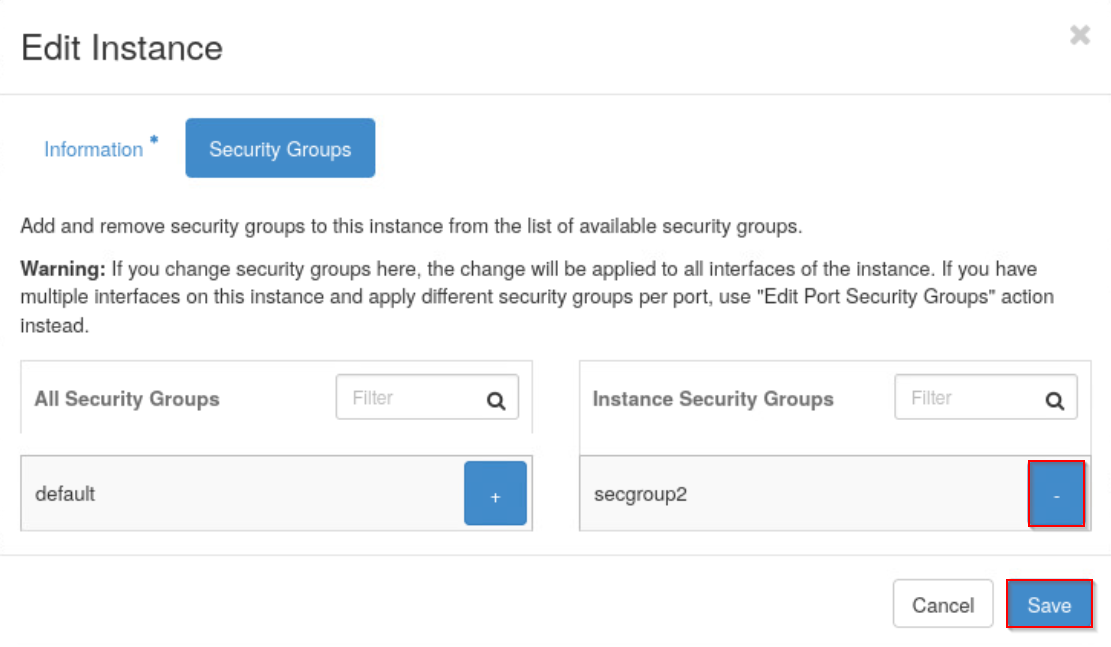
\includegraphics[width=\linewidth]{images/part2/step19.png}
        \end{center}
    \end{labstep}

    \begin{labstep}
        Re-open the popup by clicking the dropdown next to \textbf{Create Snapshot} and clicking \textbf{Edit Security Groups}.
        The \textbf{All Security Groups} list contains the security groups that are available but are not currently applied to the instance.
        Add the \textbf{default} security group to the interface by clicking the \textbf{+} button next to that group, and click \textbf{Update} to finalize the change.

        \begin{center}
            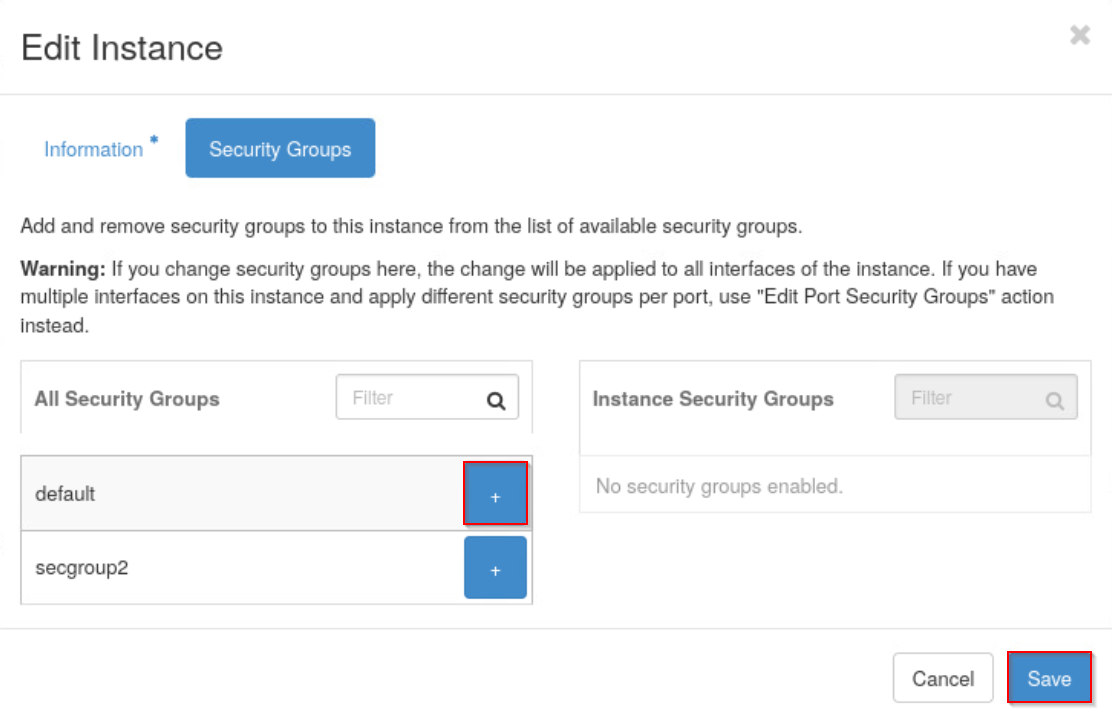
\includegraphics[width=\linewidth]{images/part2/step20.png}
        \end{center}
    \end{labstep}

    \begin{tipbox}
        You can assign and unassign multiple security groups before saving the changes.
    \end{tipbox}

    \begin{labstep}
        To verify that the security group has been applied again, click \textbf{instance1}.
        On the \textit{Overview} tab of the \textit{instance1} page, scroll down to view the \textit{Security Groups} section.
        This time, you should see the \textbf{default} security group and its rules listed.

        \begin{center}
            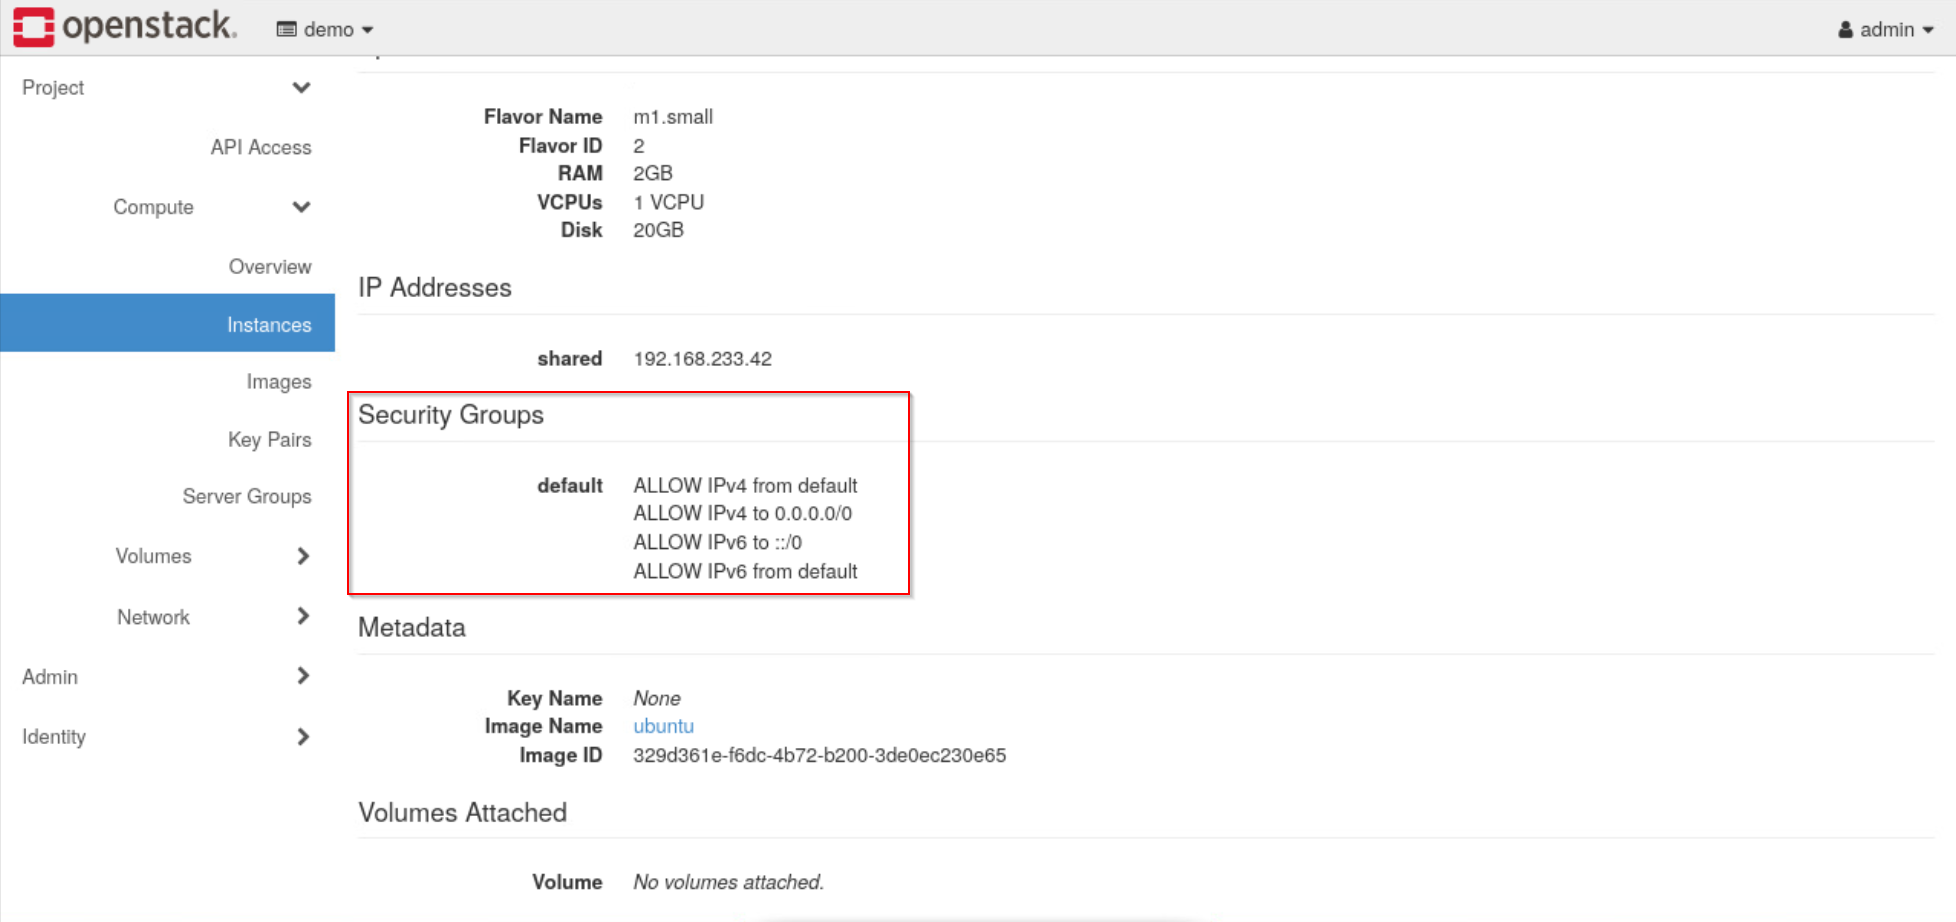
\includegraphics[width=\linewidth]{images/part2/step21.png}
        \end{center}
    \end{labstep}

    \begin{labstep}
        We no longer need this instance, so navigate back to \textbf{Project $>$ Compute $>$ Instances}, select \textbf{instance1}, and click \textbf{Delete Instances}.

        \begin{center}
            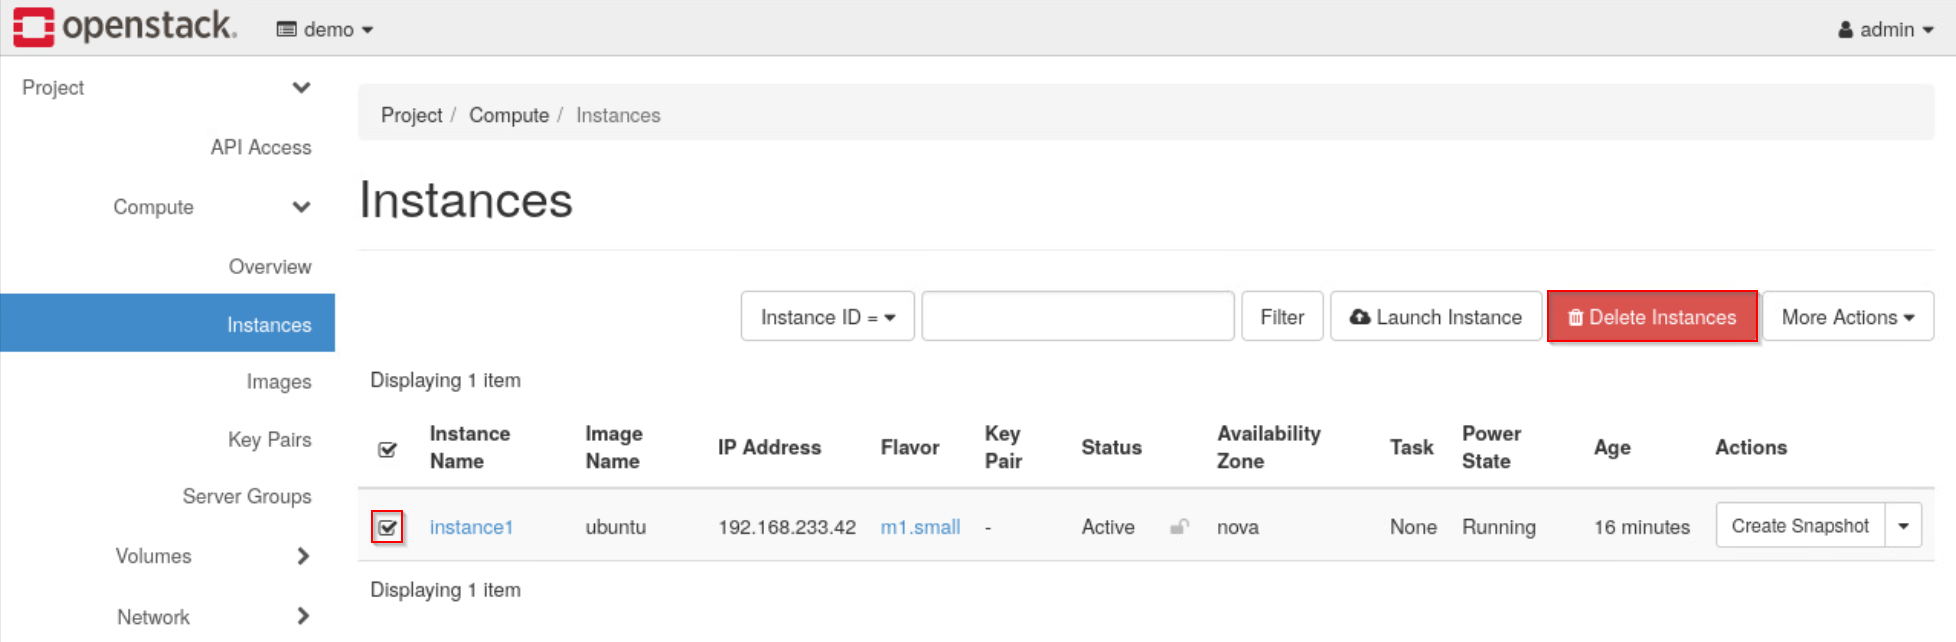
\includegraphics[width=\linewidth]{images/part2/step22.png}
        \end{center}
    \end{labstep}

    \begin{labstep}
        We will also recreate the security group in the final section of the lab in order to show a complete example, so we can safely delete \textbf{secgroup2}.
        To delete the security group from the dashboard, navigate to \textbf{Project $>$ Network $>$ Security Groups}.
        Click the dropdown next to the \textbf{Manage Rules} button in the same row as \textbf{secgroup2}, and then click \textbf{Delete Security Group}.

        \begin{center}
            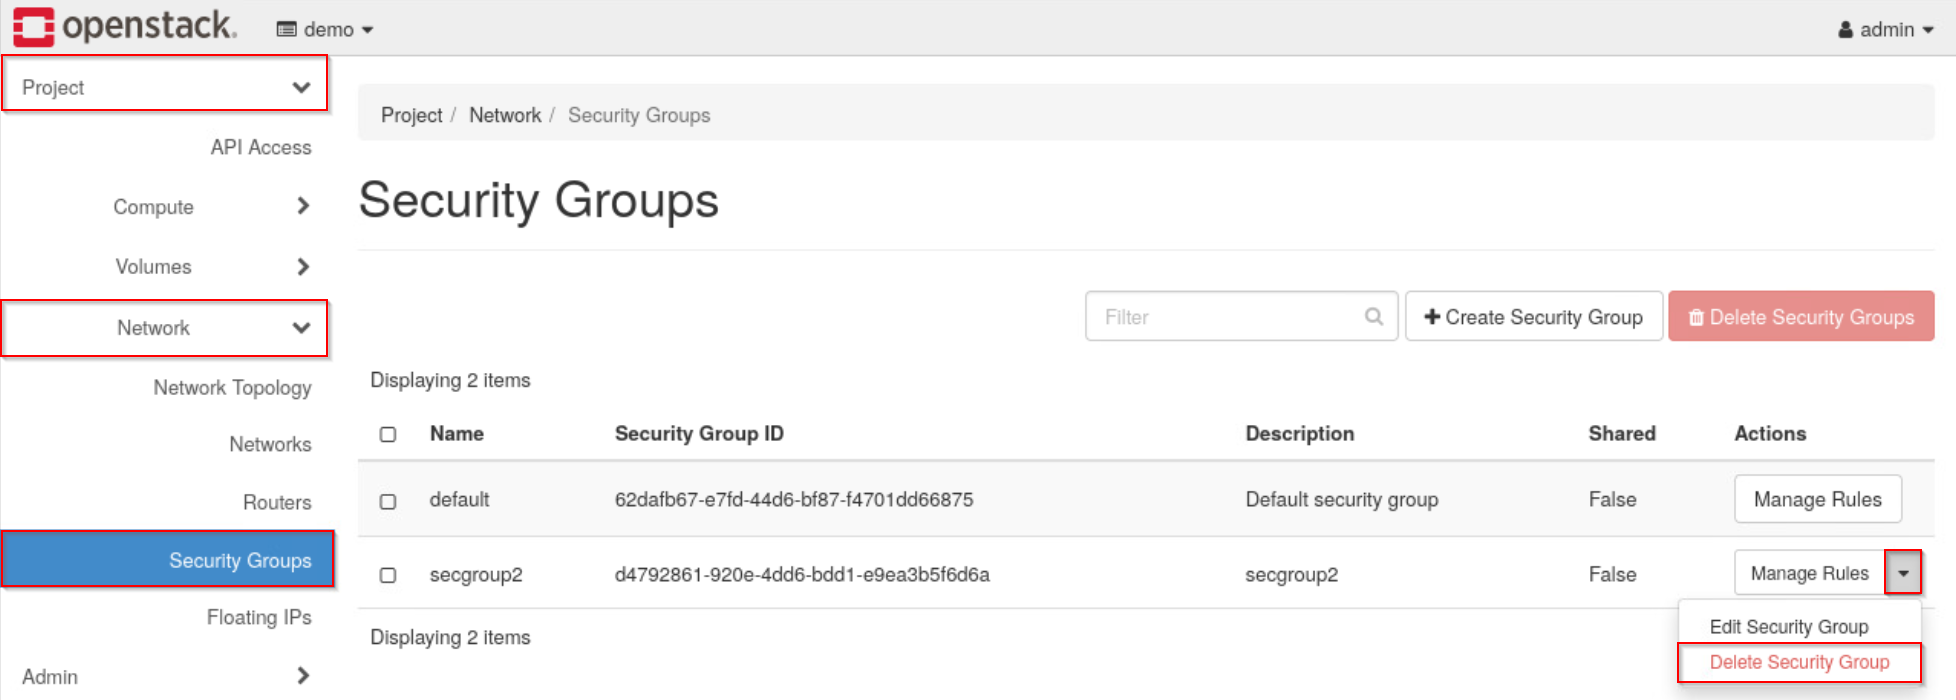
\includegraphics[width=\linewidth]{images/part2/step23.png}
        \end{center}
    \end{labstep}

    \begin{labstep}
        Leave the web browser open, and continue to the next task.
    \end{labstep}

\end{enumerate}

%%%%%%%%%%%
% Section 3
%%%%%%%%%%%
\section{Creating SSH Key Pairs}\label{sec:creating-ssh-key-pairs}
In this task, you will use the \textit{Horizon Dashboard} and \textit{OpenStack Unified CLI} to create and manage SSH key pairs.
These keys will later be used to securely connect to external instances from outside the OpenStack environment.

\begin{enumerate}
    \begin{labstep}
        If the web browser is not already open, open it.
        Navigate to \textbf{192.168.1.20}, and log in to the dashboard as \textbf{admin} with the password \textbf{secret}.

        \begin{center}
            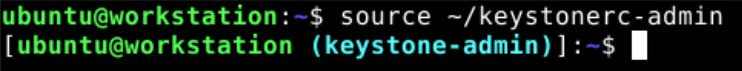
\includegraphics[scale=0.5]{images/part3/step1.png}
        \end{center}
    \end{labstep}

    \begin{labstep}
        Select the \textbf{demo} project, and navigate to \textbf{Project $>$ Compute $>$ Key Pairs}.
        Click \textbf{Create Key Pair} to create a new key pair.

        \begin{center}
            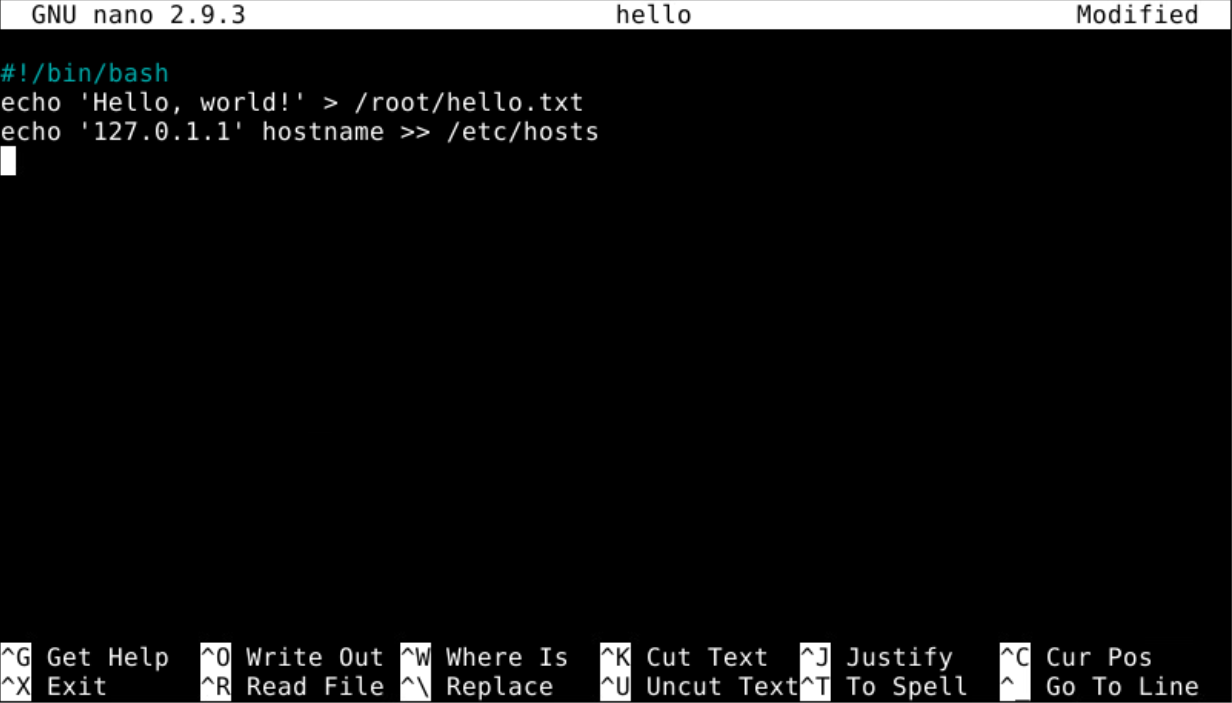
\includegraphics[width=\linewidth]{images/part3/step2.png}
        \end{center}
    \end{labstep}

    \begin{labstep}
        Enter \textbf{keypair1} in the \textit{Key Pair Name} field, and select \textbf{SSH Key} in the \textit{Key Type} dropdown.
        Click \textbf{Create Key Pair}.
        This will create the key pair and download it to the \textbf{\texttildemid/Downloads} directory.

        \begin{center}
            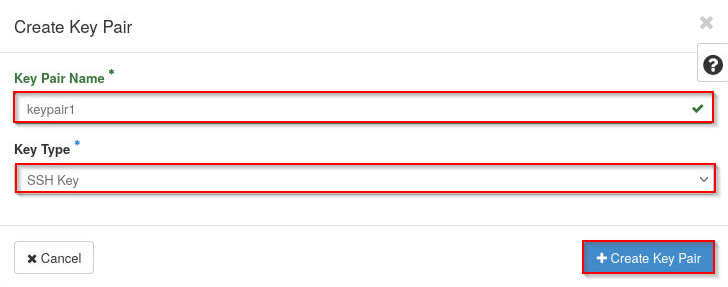
\includegraphics[width=\linewidth]{images/part3/step3.png}
        \end{center}
    \end{labstep}

    \begin{tipbox}
        When creating key pairs from the Horizon Dashboard, the private key file permissions are \textit{not} set strictly, so it is recommended to still set them through the command line.
        We will do this in the following steps.
    \end{tipbox}

    \begin{labstep}
        Sign out of the Horizon Dashboard and close the web browser.
    \end{labstep}

    \begin{labstep}
        If a terminal window is not already open, open one and source the \textbf{admin} credentials from the \textbf{\texttildemid/keystonerc-admin} file.
        \begin{lstlisting}
            ubuntu@workstation:~$ source ~/keystonerc-admin
        \end{lstlisting}

        \begin{center}
            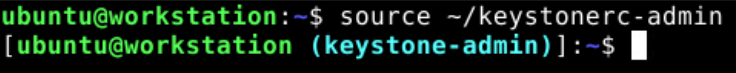
\includegraphics[width=\linewidth]{images/part3/step5.png}
        \end{center}
    \end{labstep}

    \begin{labstep}
        To better protect the private key, use the \textbf{chmod} command with a mode of \textbf{600} to make it so that the \textbf{ubuntu} user has read/write permissions on the private key file, and groups and other users have no permissions to the file.
        \begin{lstlisting}
            [ubuntu@workstation (keystone-admin)]:~$ chmod 600 ~/Downloads/keypair1.pem
        \end{lstlisting}

        \begin{center}
            \includegraphics[width=\linewidth]{images/part3/step6.png}
        \end{center}
    \end{labstep}

    \begin{labstep}
        We only need one key pair to connect to the external instance, so the key pair created from the Horizon Dashboard can safely be deleted in order to demonstrate creating a key pair from the command line.
        Delete the \textbf{keypair1} key pair.
        \begin{lstlisting}
            [ubuntu@workstation (keystone-admin)]:~$ openstack keypair delete keypair1
        \end{lstlisting}

        \begin{center}
            \includegraphics[width=\linewidth]{images/part3/step7.png}
        \end{center}
    \end{labstep}

    \begin{notebox}
        Note that a key pair in the context of OpenStack is actually a misnomer.
        The key pair object really only refers to the public key, while the private key only exists in the file in which it is saved.
        Therefore, the private key file will still exist after deleting the key pair.
    \end{notebox}

    \begin{labstep}
        Delete the private key located at \textbf{\texttildemid/Downloads/keypair1.pem}.
        \begin{lstlisting}
            [ubuntu@workstation (keystone-admin)]:~$ rm -f ~/Downloads/keypair1.pem
        \end{lstlisting}

        \begin{center}
            \includegraphics[width=\linewidth]{images/part3/step8.png}
        \end{center}
    \end{labstep}

    \begin{labstep}
        List the available key pairs to verify that \textbf{keypair1} was deleted.
        \begin{lstlisting}
            [ubuntu@workstation (keystone-admin)]:~$ openstack keypair list
        \end{lstlisting}

        \begin{center}
            \includegraphics[width=\linewidth]{images/part3/step9.png}
        \end{center}
    \end{labstep}

    \begin{labstep}
        Create the key pair \textbf{keypair2}, and save the private key to the file
        \textbf{\texttildemid/Downloads/keypair2.pem}.
        \begin{lstlisting}
            [ubuntu@workstation (keystone-admin)]:~$ openstack keypair create \
            > keypair2 > ~/Downloads/keypair2.pem
        \end{lstlisting}

        \begin{center}
            \includegraphics[width=\linewidth]{images/part3/step10.png}
        \end{center}
    \end{labstep}

    \begin{labstep}
        Set the file permissions of the private key so that only the \textbf{ubuntu} user has read/write permissions.
        \begin{lstlisting}
            [ubuntu@workstation (keystone-admin)]:~$ chmod 600 ~/Downloads/keypair2.pem
        \end{lstlisting}

        \begin{center}
            \includegraphics[width=\linewidth]{images/part3/step11.png}
        \end{center}
    \end{labstep}

    \begin{labstep}
        List the available key pairs to verify the creation of \textbf{keypair2}.
        \begin{lstlisting}
            [ubuntu@workstation (keystone-admin)]:~$ openstack keypair list
        \end{lstlisting}

        \begin{center}
            \includegraphics[width=\linewidth]{images/part3/step12.png}
        \end{center}
    \end{labstep}

    \begin{labstep}
        Leave the terminal window open and continue to the next task.
    \end{labstep}

\end{enumerate}

%%%%%%%%%%%
% Section 4
%%%%%%%%%%%
\section{Applying SSH Keys to Instances}\label{sec:applying-ssh-keys-to-instances}
In this task, you will use both the \textit{Horizon Dashboard} and \textit{OpenStack Unified CLI} to apply SSH key pairs to instances.
This is the final piece necessary to have an instance that can be reached and logged in to from an external network, which the next task will explore.

\begin{enumerate}
    \begin{labstep}
        If a terminal window is not already open, open one and source the admin credentials from the \textbf{\texttildemid/keystonerc-admin} file.
        \begin{lstlisting}
            ubuntu@workstation:~$ source ~/keystonerc-admin
        \end{lstlisting}

        \begin{center}
            \includegraphics[width=\linewidth]{images/part4/step1.png}
        \end{center}
    \end{labstep}

    \begin{labstep}
        An SSH key can be applied to an instance at creation from the command line.
        Create an instance with the \textbf{keypair2} key pair.
        \begin{lstlisting}
            [ubuntu@workstation (keystone-admin)]:~$ openstack server create \
            > --image ubuntu \
            > --flavor m1.small \
            > --network shared \
            > --key-name keypair2 \
            > instance1
        \end{lstlisting}

        \begin{center}
            \includegraphics[width=\linewidth]{images/part4/step2.png}
        \end{center}
    \end{labstep}

    \begin{tipbox}
        OpenStack does not provide a way to directly change the key pair associated with an existing instance.
        We will not need to in these labs, but if you need to use a different SSH key, one option is to manually add your new key to the \textbf{~/.ssh/authorized\_keys} file inside the instance.
        However, this change will not be tracked by OpenStack.
        Another option is to rebuild the instance with a new key pair.
        If the instance contains important data, it's important to back it up---for example, with a snapshot (covered later).
    \end{tipbox}

    \begin{labstep}
        Verify that \textbf{keypair2} is attached to \textbf{instance1}.
        \begin{lstlisting}
            [ubuntu@workstation (keystone-admin)]:~$ openstack server show \
            > -c key_name \
            > instance1
        \end{lstlisting}

        \begin{center}
            \includegraphics[width=\linewidth]{images/part4/step3.png}
        \end{center}
    \end{labstep}

    \begin{labstep}
        Delete \textbf{instance1}.
        We will recreate it from the Horizon Dashboard to demonstrate adding a security group to an instance at creation time from the dashboard.
        \begin{lstlisting}
            [ubuntu@workstation (keystone-admin)]:~$ openstack server delete instance1
        \end{lstlisting}

        \begin{center}
            \includegraphics[width=\linewidth]{images/part4/step4.png}
        \end{center}
    \end{labstep}

    \begin{labstep}
        Leave the terminal window open, and open the web browser.
        Navigate to \textbf{192.168.1.20}, and log in to the dashboard as \textbf{admin} with the password \textbf{secret}.

        \begin{center}
            \includegraphics[scale=0.5]{images/part4/step5.png}
        \end{center}
    \end{labstep}

    \begin{labstep}
        Select the \textbf{demo} project.
        Navigate to \textbf{Project $>$ Compute $>$ Instances}, and click \textbf{Launch Instance}.

        \begin{center}
            \includegraphics[width=\linewidth]{images/part4/step6.png}
        \end{center}
    \end{labstep}

    \begin{labstep}
        In the \textit{Details} tab, type \textbf{instance1} in the \textit{Instance Name} field.
        Click \textbf{Next}.

        \begin{center}
            \includegraphics[width=\linewidth]{images/part4/step7.png}
        \end{center}
    \end{labstep}

    \begin{labstep}
        In the \textit{Source} tab, set \textit{Create New Volume} to \textbf{No}, and scroll down (if needed) to select the \textbf{ubuntu} image.
        Click \textbf{Next}.

        \begin{center}
            \includegraphics[width=\linewidth]{images/part4/step8.png}
        \end{center}
    \end{labstep}

    \begin{stopbox}
        Before proceeding to the next step, confirm that \textbf{ubuntu} appears in the \textit{Allocated} section.
    \end{stopbox}

    \begin{labstep}
        In the \textit{Flavor} tab, scroll down (if needed) to select the \textbf{m1.small} flavor.
        Click \textbf{Next}.

        \begin{center}
            \includegraphics[width=\linewidth]{images/part4/step9.png}
        \end{center}
    \end{labstep}

    \begin{stopbox}
        Before proceeding to the next step, confirm that \textbf{m1.small} appears in the \textit{Allocated} section.
    \end{stopbox}

    \begin{labstep}
        In the \textit{Networks} tab, select the \textbf{shared} network.
        Navigate to the \textit{Key Pair} tab.

        \begin{center}
            \includegraphics[width=\linewidth]{images/part4/step10.png}
        \end{center}
    \end{labstep}

    \begin{stopbox}
        Before proceeding to the next step, confirm that \textbf{shared} appears in the \textit{Allocated} section.
    \end{stopbox}

    \begin{labstep}
        In the \textit{Key Pair} tab, select \textbf{keypair2} if it is not already in the \textit{Allocated} section, and click \textbf{Launch Instance}.

        \begin{center}
            \includegraphics[width=\linewidth]{images/part4/step11.png}
        \end{center}
    \end{labstep}

    \begin{stopbox}
        Before proceeding to the next step, confirm that \textbf{keypair2} appears in the \textit{Allocated} section.
    \end{stopbox}

    \begin{labstep}
        You should be redirected to the \textbf{Project $>$ Compute $>$ Instances} page.
        To verify that the key pair was applied, first click \textbf{instance1} to go to the instance's details page.

        \begin{center}
            \includegraphics[width=\linewidth]{images/part4/step12.png}
        \end{center}
    \end{labstep}

    \begin{labstep}
        Scroll down to the \textit{Metadata} section and verify that \textbf{keypair2} is present in the \textit{Key Name} row.

        \begin{center}
            \includegraphics[width=\linewidth]{images/part4/step13.png}
        \end{center}
    \end{labstep}

    \begin{notebox}
        If an instance does not have a key pair, the \textit{Key Name} row will show ``None''.
    \end{notebox}

    \begin{labstep}
        We no longer need this instance, so navigate back to \textbf{Project $>$ Compute $>$ Instances}, select \textbf{instance1}, and click \textbf{Delete Instances}.

        \begin{center}
            \includegraphics[width=\linewidth]{images/part4/step14.png}
        \end{center}
    \end{labstep}

    \begin{labstep}
        We will also recreate the key pair in the final section of the lab in order to show a complete example.
        So, we can safely delete \textbf{keypair2}.
        To delete the key pair from the dashboard, navigate to \textbf{Project $>$ Compute $>$ Key Pairs}, and click the \textbf{Delete Key Pair} button in the same row as \textbf{keypair2}.

        \begin{center}
            \includegraphics[width=\linewidth]{images/part4/step15.png}
        \end{center}
    \end{labstep}

    \begin{labstep}
        Log out of the \textit{Horizon Dashboard}, and close the web browser.
        Continue to the next task.
    \end{labstep}

\end{enumerate}

%%%%%%%%%%%
% Section 5
%%%%%%%%%%%
\section{Launching and Verifying an External Instance}\label{sec:launching-an-external-instance}
Up to this point, you have learned how to create an external network, a router, a floating IP address, an SSH key pair, and a security group.
These are all the resources necessary to create and interact with an external instance from outside the OpenStack cloud.
In this task, you will put all these concepts together to create a functioning external instance.
You will create the necessary resources, launch an external instance, and verify its connectivity and functionality with the \textbf{ssh} and \textbf{ping} commands.

\begin{enumerate}
    \begin{labstep}
        If a terminal window is not already open, open one and source the admin credentials from the \textbf{\texttildemid/keystonerc-admin} file.
        \begin{lstlisting}
            ubuntu@workstation:~$ source ~/keystonerc-admin
        \end{lstlisting}

        \begin{center}
            \includegraphics[width=\linewidth]{images/part5/step1.png}
        \end{center}
    \end{labstep}

    \begin{labstep}
        Before creating our own router and external network, we need to delete the ones that are created by default.
        First, unset the external gateway from \textbf{router1}.
        \begin{lstlisting}
            [ubuntu@workstation (keystone-admin)]:~$ openstack router unset \
            > --external-gateway \
            > router1
        \end{lstlisting}

        \begin{center}
            \includegraphics[width=\linewidth]{images/part5/step2.png}
        \end{center}
    \end{labstep}

    \begin{labstep}
        List the interfaces of \textbf{router1}.
        \begin{lstlisting}
            [ubuntu@workstation (keystone-admin)]:~$ openstack port list \
            > -c ID \
            > -f value \
            > --router router1
        \end{lstlisting}

        \begin{center}
            \includegraphics[width=\linewidth]{images/part5/step3.png}
        \end{center}
    \end{labstep}

    \begin{labstep}
        Capture the output of the previous command in to a variable called \textbf{ports}.
        \begin{lstlisting}
            [ubuntu@workstation (keystone-admin)]:~$ ports=$(!!)
        \end{lstlisting}

        \begin{center}
            \includegraphics[width=\linewidth]{images/part5/step4.png}
        \end{center}
    \end{labstep}

    \begin{labstep}
        Ensure that \textbf{ports} contains the ID values as expected.
        \begin{lstlisting}
            [ubuntu@workstation (keystone-admin)]:~$ echo $ports
        \end{lstlisting}

        \begin{center}
            \includegraphics[width=\linewidth]{images/part5/step5.png}
        \end{center}
    \end{labstep}

    \begin{labstep}
        Remove the interfaces from \textbf{router1}.
        \begin{lstlisting}
            [ubuntu@workstation (keystone-admin)]:~$ for port in $ports; do \
            > openstack router remove port router1 $port; \
            > done
        \end{lstlisting}

        \begin{center}
            \includegraphics[width=\linewidth]{images/part5/step6.png}
        \end{center}
    \end{labstep}

    \begin{labstep}
        Delete \textbf{router1}.
        \begin{lstlisting}
            [ubuntu@workstation (keystone-admin)]:~$ openstack router delete router1
        \end{lstlisting}

        \begin{center}
            \includegraphics[width=\linewidth]{images/part5/step7.png}
        \end{center}
    \end{labstep}

    \begin{labstep}
        Delete the \textbf{public} network.
        \begin{lstlisting}
            [ubuntu@workstation (keystone-admin)]:~$ openstack network delete public
        \end{lstlisting}

        \begin{center}
            \includegraphics[width=\linewidth]{images/part5/step8.png}
        \end{center}
    \end{labstep}

    \begin{labstep}
        First, we will create an external network.
        List the existing networks to ensure that one does not already exist.
        Only the \textbf{shared} and \textbf{private} networks should be listed in the output.
        \begin{lstlisting}
            [ubuntu@workstation (keystone-admin)]:~$ openstack network list
        \end{lstlisting}

        \begin{center}
            \includegraphics[width=\linewidth]{images/part5/step9.png}
        \end{center}
    \end{labstep}

    \begin{labstep}
        Create an external network named \textbf{external}.
        Set the network type to \textbf{flat} and the physical network to \textbf{public}.
        Set the network as shared and external.
        \begin{lstlisting}
            [ubuntu@workstation (keystone-admin)]:~$ openstack network create \
            > --external \
            > --share \
            > --provider-network-type flat \
            > --provider-physical-network public \
            > external
        \end{lstlisting}

        \begin{center}
            \includegraphics[width=\linewidth]{images/part5/step10.png}
        \end{center}
    \end{labstep}

    \begin{labstep}
        Create a subnet named \textbf{external-subnet} in the \textbf{external} network.
        Give the subnet a range of \textbf{172.25.250.60} to \textbf{172.25.250.80}.
        Disable DHCP services for the subnet, and use the address \textbf{172.25.250.254} as the gateway and the DNS name server.
        \begin{lstlisting}
            [ubuntu@workstation (keystone-admin)]:~$ openstack subnet create \
            > --subnet-range 172.25.250.0/24 \
            > --no-dhcp \
            > --gateway 172.25.250.254 \
            > --dns-nameserver 172.25.250.254 \
            > --allocation-pool start=172.25.250.60,end=172.25.250.80 \
            > --network external \
            > external-subnet
        \end{lstlisting}

        \begin{center}
            \includegraphics[width=\linewidth]{images/part5/step11.png}
        \end{center}
    \end{labstep}

    \begin{labstep}
        List the networks again to verify the creation of the \textbf{external} network.
        \begin{lstlisting}
            [ubuntu@workstation (keystone-admin)]:~$ openstack network list
        \end{lstlisting}

        \begin{center}
            \includegraphics[width=\linewidth]{images/part5/step12.png}
        \end{center}
    \end{labstep}

    \begin{labstep}
        List the existing routers.
        The output should be empty.
        \begin{lstlisting}
            [ubuntu@workstation (keystone-admin)]:~$ openstack router list
        \end{lstlisting}

        \begin{center}
            \includegraphics[width=\linewidth]{images/part5/step13.png}
        \end{center}
    \end{labstep}

    \begin{labstep}
        Next, create a router named \textbf{router-external}.
        \begin{lstlisting}
            [ubuntu@workstation (keystone-admin)]:~$ openstack router create router-external
        \end{lstlisting}

        \begin{center}
            \includegraphics[width=\linewidth]{images/part5/step14.png}
        \end{center}
    \end{labstep}

    \begin{labstep}
        List the routers again to verify the creation of \textbf{router-external}.
        \begin{lstlisting}
            [ubuntu@workstation (keystone-admin)]:~$ openstack router list
        \end{lstlisting}

        \begin{center}
            \includegraphics[width=\linewidth]{images/part5/step15.png}
        \end{center}
    \end{labstep}

    \begin{labstep}
        The router needs to be connected to both the \textbf{shared-subnet} and \textbf{external-subnet} networks to allow external connections to the instance.
        First, add the \textbf{shared-subnet} to the router.
        \begin{lstlisting}
            [ubuntu@workstation (keystone-admin)]:~$ openstack router add subnet \
            > router-external \
            > shared-subnet
        \end{lstlisting}

        \begin{center}
            \includegraphics[width=\linewidth]{images/part5/step16.png}
        \end{center}
    \end{labstep}

    \begin{labstep}
        Set the \textbf{external} network as the gateway for the router.
        \begin{lstlisting}
            [ubuntu@workstation (keystone-admin)]:~$ openstack router set \
            > --external-gateway external \
            > router-external
        \end{lstlisting}

        \begin{center}
            \includegraphics[width=\linewidth]{images/part5/step17.png}
        \end{center}
    \end{labstep}

    \begin{labstep}
        Show the details of \textbf{router-external} to show that it is connected to two subnets.
        \begin{lstlisting}
            [ubuntu@workstation (keystone-admin)]:~$ openstack router show router-external
        \end{lstlisting}

        \begin{center}
            \includegraphics[width=\linewidth]{images/part5/step18.png}
        \end{center}
    \end{labstep}

    \begin{labstep}
        Now, we will create a floating IP address to associate with the instance.
        This will be the IP address we use to connect to the instance through the \textbf{external} network.
        First, list the available floating IP addresses.
        The output should be empty.
        \begin{lstlisting}
            [ubuntu@workstation (keystone-admin)]:~$ openstack floating ip list
        \end{lstlisting}

        \begin{center}
            \includegraphics[width=\linewidth]{images/part5/step19.png}
        \end{center}
    \end{labstep}

    \begin{labstep}
        Create the floating IP address \textbf{172.25.250.75} in the \textbf{external} network.
        \begin{lstlisting}
            [ubuntu@workstation (keystone-admin)]:~$ openstack floating ip create \
            > --floating-ip-address 172.25.250.75 \
            > external
        \end{lstlisting}

        \begin{center}
            \includegraphics[width=\linewidth]{images/part5/step20.png}
        \end{center}
    \end{labstep}

    \begin{labstep}
        List the floating IP addresses again to verify the creation of \textbf{172.25.250.75}.
        \begin{lstlisting}
            [ubuntu@workstation (keystone-admin)]:~$ openstack floating ip list
        \end{lstlisting}

        \begin{center}
            \includegraphics[width=\linewidth]{images/part5/step21.png}
        \end{center}
    \end{labstep}

    \begin{labstep}
        In order for our ICMP and SSH requests to reach our external instance, we need to set up a security group and security rules that allow this traffic.
        First, list the available security groups.
        The output should contain two default security groups.
        \begin{lstlisting}
            [ubuntu@workstation (keystone-admin)]:~$ openstack security group list
        \end{lstlisting}

        \begin{center}
            \includegraphics[width=\linewidth]{images/part5/step22.png}
        \end{center}
    \end{labstep}

    \begin{labstep}
        Create a security group.
        Because we will allow ICMP and SSH traffic, we will name the security group \textbf{sg-allow-icmp-ssh}.
        \begin{lstlisting}
            [ubuntu@workstation (keystone-admin)]:~$ openstack security group create \
            > sg-allow-icmp-ssh
        \end{lstlisting}

        \begin{center}
            \includegraphics[width=\linewidth]{images/part5/step23.png}
        \end{center}
    \end{labstep}

    \begin{tipbox}
        Real-world OpenStack environments may have a variety of instances with different security group needs.
        Therefore, it pays to be descriptive in your naming conventions so that you can more easily identify the appropriate security group later.
        It is much easier to tell what \textbf{sg-allow-icmp-ssh} does than it is to guess the purpose of \textbf{secgroup1}.
        However, giving strong names alone is not enough---it is always best to check a security group's actual rules before adding it to an instance.
    \end{tipbox}

    \begin{labstep}
        List the security groups to verify the creation of \textbf{sg-allow-icmp-ssh}.
        \begin{lstlisting}
            [ubuntu@workstation (keystone-admin)]:~$ openstack security group list
        \end{lstlisting}

        \begin{center}
            \includegraphics[width=\linewidth]{images/part5/step24.png}
        \end{center}
    \end{labstep}

    \begin{labstep}
        List the rules in the \textbf{sg-allow-icmp-ssh} security group.
        There should be two rules created by default.
        \begin{lstlisting}
            [ubuntu@workstation (keystone-admin)]:~$ openstack security group rule list \
            > sg-allow-icmp-ssh
        \end{lstlisting}

        \begin{center}
            \includegraphics[width=\linewidth]{images/part5/step25.png}
        \end{center}
    \end{labstep}

    \begin{tipbox}
        Try to use the \textbf{for} loop trick to verify that the default security rules allow IPv4 and IPv6 egress traffic.
        You can use this command to show the details of a rule:
        \begin{lstlisting}
            openstack security group rule show <ID>
        \end{lstlisting}
    \end{tipbox}

    \begin{labstep}
        Add a security rule in the \textbf{sg-allow-icmp-ssh} security group to allow all incoming ICMP traffic.
        \begin{lstlisting}
            [ubuntu@workstation (keystone-admin)]:~$ openstack security group rule create \
            > --protocol icmp \
            > sg-allow-icmp-ssh
        \end{lstlisting}

        \begin{center}
            \includegraphics[scale=0.45]{images/part5/step26.png}
        \end{center}
    \end{labstep}

    \begin{labstep}
        Add another security rule to allow remote connection using SSH on the default port 22.
        \begin{lstlisting}
            [ubuntu@workstation (keystone-admin)]:~$ openstack security group rule create \
            > --protocol tcp \
            > --dst-port 22 \
            > sg-allow-icmp-ssh
        \end{lstlisting}

        \begin{center}
            \includegraphics[scale=0.45]{images/part5/step27.png}
        \end{center}
    \end{labstep}

    \begin{labstep}
        List the rules of the \textbf{sg-allow-icmp-ssh} security group again to verify that there are now four rules: the two default rules plus the two rules you just added.
        \begin{lstlisting}
            [ubuntu@workstation (keystone-admin)]:~$ openstack security group rule list \
            > sg-allow-icmp-ssh
        \end{lstlisting}

        \begin{center}
            \includegraphics[width=\linewidth]{images/part5/step28.png}
        \end{center}
    \end{labstep}

    \begin{labstep}
        Finally, we need an SSH key pair to remotely log in to the external instance.
        List the available key pairs.
        The output should be empty.
        \begin{lstlisting}
            [ubuntu@workstation (keystone-admin)]:~$ openstack keypair list
        \end{lstlisting}

        \begin{center}
            \includegraphics[width=\linewidth]{images/part5/step29.png}
        \end{center}
    \end{labstep}

    \begin{labstep}
        Create a key pair called \textbf{keypair}, and save the private key to \textbf{~/Downloads/keypair.pem}.
        \begin{lstlisting}
            [ubuntu@workstation (keystone-admin)]:~$ openstack keypair create \
            > keypair > ~/Downloads/keypair.pem
        \end{lstlisting}

        \begin{center}
            \includegraphics[width=\linewidth]{images/part5/step30.png}
        \end{center}
    \end{labstep}

    \begin{labstep}
        Set the file permissions of the private key so that only the \textbf{ubuntu} user has read/write permissions.
        \begin{lstlisting}
            [ubuntu@workstation (keystone-admin)]:~$ chmod 600 ~/Downloads/keypair.pem
        \end{lstlisting}

        \begin{center}
            \includegraphics[width=\linewidth]{images/part5/step31.png}
        \end{center}
    \end{labstep}

    \begin{labstep}
        List the available key pairs again to verify the creation of \textbf{keypair}.
        \begin{lstlisting}
            [ubuntu@workstation (keystone-admin)]:~$ openstack keypair list
        \end{lstlisting}

        \begin{center}
            \includegraphics[width=\linewidth]{images/part5/step32.png}
        \end{center}
    \end{labstep}

    \begin{labstep}
        We now have all the resources we need to create an external instance.
        List all instances in the project.
        The output should be empty.
        \begin{lstlisting}
            [ubuntu@workstation (keystone-admin)]:~$ openstack server list
        \end{lstlisting}

        \begin{center}
            \includegraphics[width=\linewidth]{images/part5/step33.png}
        \end{center}
    \end{labstep}

    \begin{labstep}
        Launch an instance named \textbf{instance-external} with the \textbf{ubuntu} image, the \textbf{m1.small} flavor, the \textbf{keypair2} key pair, the \textbf{shared} network, and the \textbf{secgroup2} security group.
        \begin{lstlisting}
            [ubuntu@workstation (keystone-admin)]:~$ openstack server create \
            > --image ubuntu \
            > --flavor m1.small \
            > --network shared \
            > --security-group sg-allow-icmp-ssh \
            > --key-name keypair \
            > instance-external
        \end{lstlisting}

        \begin{center}
            \includegraphics[width=\linewidth]{images/part5/step34.png}
        \end{center}
    \end{labstep}

    \begin{labstep}
        List the floating IPs.
        \begin{lstlisting}
            [ubuntu@workstation (keystone-admin)]:~$ openstack floating ip list
        \end{lstlisting}

        \begin{center}
            \includegraphics[width=\linewidth]{images/part5/step35.png}
        \end{center}
    \end{labstep}

    \begin{labstep}
        Associate the floating IP address with the \textbf{instance-external} instance.
        \begin{lstlisting}
            [ubuntu@workstation (keystone-admin)]:~$ openstack server add floating ip \
            > instance-external \
            > 172.25.250.75
        \end{lstlisting}

        \begin{center}
            \includegraphics[width=\linewidth]{images/part5/step36.png}
        \end{center}
    \end{labstep}

    \begin{labstep}
        Verify that the instance was assigned the floating IP address.
        \begin{lstlisting}
            [ubuntu@workstation (keystone-admin)]:~$ openstack server list \
            > -c Name \
            > -c Networks
        \end{lstlisting}

        \begin{center}
            \includegraphics[width=\linewidth]{images/part5/step37.png}
        \end{center}
    \end{labstep}

    \begin{labstep}
        Use the \textbf{scp} command to send the \textbf{keypair2} key pair to the \textbf{devstack} machine over SSH.
        Use the password \textbf{ubuntu} for authentication.
        \begin{lstlisting}
            [ubuntu@workstation (keystone-admin)]:~$ scp ~/Downloads/keypair.pem \
            > 192.168.1.20:~/keypair.pem
        \end{lstlisting}

        \begin{center}
            \includegraphics[width=\linewidth]{images/part5/step38.png}
        \end{center}
    \end{labstep}

    \begin{notebox}
        Because your username is \textbf{ubuntu} on both machines, you don't need to specify the username in the \textbf{scp} command.
        By default, \textbf{scp} uses your current local username for the remote connection.
        If you wanted to send the file to a different user, such as \textbf{user2} on the \textbf{devstack} machine, you would write: \textbf{user2@192.168.1.20:\texttildemid/keypair.pem}.
    \end{notebox}

    \begin{labstep}
        SSH into the \textbf{devstack} machine.
        Use the password \textbf{ubuntu} when prompted.
        \begin{lstlisting}
            [ubuntu@workstation (keystone-admin)]:~$ ssh 192.168.1.20
        \end{lstlisting}

        \begin{center}
            \includegraphics[width=\linewidth]{images/part5/step39.png}
        \end{center}
    \end{labstep}

    \begin{labstep}
        Ping the \textbf{instance-external} instance with the floating IP that was assigned to it in the previous task.
        This will verify that the instance can be reached and that its security group allows ICMP ingress traffic.
        \begin{lstlisting}
            ubuntu@devstack:~$ ping -c3 172.25.250.75
        \end{lstlisting}

        \begin{center}
            \includegraphics[width=\linewidth]{images/part5/step40.png}
        \end{center}
    \end{labstep}

    \begin{notebox}
        You should receive three successful ping replies.
    \end{notebox}

    \begin{labstep}
        SSH into the \textbf{instance-external} instance with the \textbf{keypair2.pem} file.
        Enter \textbf{yes} when asked if you want to continue.
        \begin{lstlisting}
            ubuntu@devstack:~$ ssh -i ~/keypair2.pem \
            > 172.25.250.75
        \end{lstlisting}

        \begin{center}
            \includegraphics[width=\linewidth]{images/part5/step41.png}
        \end{center}
    \end{labstep}

    \begin{notebox}
        It may take a few minutes for the instance to be fully booted and ready to accept SSH connections.
    \end{notebox}
    \begin{notebox}
        It is important to connect to the instance through SSH from the \textbf{devstack} machine since it is outside the OpenStack cloud.
        A successful connection verifies the external connectivity of the instance.
    \end{notebox}

    \begin{labstep}
        Ping the DHCP server on the \textbf{shared} network to verify connectivity.
        \begin{lstlisting}
            ubuntu@instance-external:~$ ping -c3 192.168.233.2
        \end{lstlisting}

        \begin{center}
            \includegraphics[width=\linewidth]{images/part5/step42.png}
        \end{center}
    \end{labstep}

    \begin{notebox}
        You should receive three successful ping replies.
    \end{notebox}

    \begin{labstep}
        The lab is now complete.
    \end{labstep}

\end{enumerate}

%%%%%%%%%%%%
% Appendix A
%%%%%%%%%%%%
\appendix
\section{Fine-Grained Security Group Control}
In Section~\ref{sec:applying-security-groups-to-instances}, we discussed applying security groups to instances.
However, in reality, security groups are applied to the individual ports on an instance.
For simplicity, we could mostly ignore this distinction and treat them as if they applied directly to the instance.
More fine-grained control over security groups is available from both the CLI and web interface, which is especially useful when working with instances that have multiple interfaces that each have different requirements.

From the dashboard, managing security groups for individual ports only requires navigating a new menu.
In Section~\ref{sec:applying-security-groups-to-instances}, Step~\ref{it:secgroup}, we clicked \textbf{Edit Security Groups} in the instance's dropdown menu.
To manage security groups for a specific interface instead, click \textbf{Edit Port Security Groups}.
The interface is nearly identical.

From the CLI, working with individual ports requires slightly different commands.
The following commands apply to the \textit{entire} instance---that is, to all its ports (with some exceptions):
\begin{lstlisting}
    openstack server add security group <instance> <security_group>
    openstack server remove security group <instance> <security_group>
\end{lstlisting}

Security groups can also be managed for each port from the CLI; however, the process can be slightly more cumbersome because unnamed ports must be specified by ID.

First, it is recommended to maximize your terminal window to prevent ID values from being split across lines.
This will make it easier to copy the IDs to the clipboard.
View the ports of an instance to get their IDs.
\begin{lstlisting}
    openstack port list --server <instance_name_or_id>
\end{lstlisting}
\noindent
For each port you want to modify, first copy its ID to the clipboard.
Alternatively, use the ID to name the port with
\begin{lstlisting}
    openstack port set --name <new_port_name> <port_name_or_id>
\end{lstlisting}
\noindent
or name a port upon creation with
\begin{lstlisting}
    openstack port create --name <port_name> --network <network_name_or_id>
\end{lstlisting}
\noindent
Next, find the security groups applied to the port.
\begin{lstlisting}
    openstack port show <port_name_or_id> -c security_group_ids
\end{lstlisting}
\noindent
Optionally, find the name of each security group.
\begin{lstlisting}
    openstack security group show <security_group_id> -c name
\end{lstlisting}
\noindent
Finally, remove a security group from an interface individually with
\begin{lstlisting}
    openstack port unset --security-group <security_group_name_or_id> <port_name_or_id>
\end{lstlisting}
\noindent
or remove all security groups from an interface with
\begin{lstlisting}
    openstack port set --no-security-group <port_name_or_id>
\end{lstlisting}

\end{document}
